%%%%%%%%%%%%%%%%%%%%%%%%%%%%%%%%%%%%%%%%%%%%%%%%%%%%%%%%%%%%%%%%%%%%%%%%%%%%%%%%
% This is the Mamba user manual Tex source

\documentclass[a4paper,10pt,oneside]{article}
\usepackage[table]{xcolor}
\usepackage{mamba}

\title{Mamba Image User Manual}
\author{Nicolas BEUCHER \and Serge BEUCHER}
\date{\today}

%%%%%%%%%%%%%%%%%%%%%%%%%%%%%%%%%%%%%%%%%%%%%%%%%%%%%%%%%%%%%%%%%%%%%%%%%%%%%%%%
% Document

\begin{document}

\mambaCover
\mambaContent
\mambaFigures

\section{Introduction}

This document is the user manual of the library for Python \textbf{Mamba Image}.

Mamba Image is a mathematical morphology library, its name actually stands for 
\textbf{MA}thematical \textbf{M}orphology li\textbf{B}r\textbf{A}ry \textbf{Image} 
(For sake of simplicity, the library will be referred to as Mamba). The library 
provides a wide set of functions needed to perform common operations used in 
mathematical morphology like erosion, dilation, etc... but also more complex ones
(geodesic operators, watershed transformations...).

Before reading this document, make sure you have a basic knowledge of the Python
programming language (see the Python tutorial at 
\url{http://docs.python.org/tutorial/}) and that you know the basics of 
mathematical morphology (online courses are available at 
\url{http://cmm.ensmp.fr/~serra/acours.htm} and \url{http://cmm.ensmp.fr/~beucher/publi.html}).

This document addresses various points to help you understand how to use and
enjoy Mamba, such as getting familiar with it, what it does and does not,
understand how the library works, what you can do to optimize it for your
needs. If you are new to it, read the next section, quick start, before going
further.

This is the user manual of version 2 of the library. If you were a Mamba 1 or
1.1 user, please read the section \ref{cha:change_mamba2}. Many changes
were introduced in this version and this section will help you know what to
expect.

\pagebreak

\section{A quick start}

For all intent and purpose, we will now assume that you know what mathematical
morphology is, at least theoretically (and your interest in Mamba is to go 
practical), and that you have a minimum know-how in programming with Python.

We are aware that fulfilling these two conditions may be quite difficult. It is 
likely you know one and not the other. The present authors were unable to 
fulfil them when the project Mamba started. So don't get discouraged if you are
not yet familiar with one aspect or the other. There is plenty information over
the web to get you started on either one. This document is not intended to serve
as a mathematical morphology course nor as a programming lesson as these goals are
beyond our time or ability to perform. However, we list at the end of the
document (see appendix \ref{cha:to_go_further}) various websites or pdf documents which are 
accessible online that can provide you with this information. Of course, we hope that
Mamba will give you the incentive to learn one aspect or the other to solve
any image analysis problem you may have (see our examples to see the 
possibilities offered by such a tool).

To get started with Mamba, you need to install some software on your PC. The 
most obvious one is Python. You can find Python at \url{http://www.Python.org}. 
Download version 2.7 or 3.4 and install it. Once Python is installed, you will
need to download the lastest version of the Python Imaging Library fork, Pillow
(standard PIL may not work, we do test Mamba only with Pillow) at 
\url{https://pypi.python.org/pypi/Pillow/}.
You need to download the version corresponding to your version of Python (this
should be indicated in the name of the file). Again install it. On Linux, you may
have to install the Tkinter library if it was not provided with your Python
distribution (Windows users don't need to worry as it is part of the standard 
Python distribution they just installed). Finally download the Mamba library 
from \url{http://www.mamba-image.org} (as for Pillow, select the version corresponding
to your Python version) and install it.

These instructions may not be interpreted in the same way depending on your 
system specification. If you need more information refer to section
\ref{cha:inst_comp}.

At this point your PC is now equipped with every piece of software it needs to
use Mamba, so let's get started.

First, we will show you how to launch Mamba and use it in your programs.
To use Mamba, simply type in your Python console:

\lstset{language=Python}
\begin{lstlisting}
from mamba import * 
\end{lstlisting}

This import gives you direct access to all the functions needed to 
perform basic and advanced operations found in every mathematical
morphology algorithm on 2D images.

The 3D operators can be accessed through the following import:

\lstset{language=Python}
\begin{lstlisting}
from mamba3D import *
\end{lstlisting}

\tipBox{
If you are using Windows, you can start more easily by clicking on the created
Mamba Shell shortcut in your start menu. It will launch an IDLE (the standard
Python shell on Windows) with preloaded Mamba modules and packages and some 
default images created. If you are an IDLE user, this is the
recommanded way (see section \ref{cha:lim_restrict} for more information
regarding Mamba and IDLE).
}

You now have all the tools offered in Mamba loaded on your computer and you are
ready to try your ideas. Obviously you have some image that you would like to
process, so naturally the very first step is to load it into your program.

\lstset{language=Python}
\begin{lstlisting}
# Replace the "path/to/your/image" by the correct path
im = imageMb("path/to/your/image")
\end{lstlisting}

At this point, you can manipulate your image using the reference im. For example,
you could try to get some information about this image:

\lstset{language=Python}
\begin{lstlisting}
# Printing the size of the image (width, height)
print(im.getSize())
# Printing the depth of the image 
print(im.getDepth())
\end{lstlisting}

The first thing you may notice is that the returned image size is not the actual
image size (as it is registered when you look into the image properties). For
performance sake, Mamba can only work with images that have a width multiple of 64
and a height multiple of 2. If not, the image is automatically padded. You can 
also notice that your image was put into a greyscale image (the second command 
returns 8 which means 8 bits per pixel, the image pixels can take 256 values, from 
0 to 255). Depth can be 1 bit per pixel, 8 bits per pixel or 32 bits per pixel.

Well, this is all interesting but it does not give you access to the primary
properties of an image i.e. how it looks like. To do so, Mamba gives you access to
an embedded image displayer. You can call it for every image you create.

\lstset{language=Python}
\begin{lstlisting}
im.show()
\end{lstlisting}

This should have created a window displaying your image. There is no color
obviously because your image was transformed into a greyscale image upon loading.

The display comes with lots of options and possibilities to help you visualize
your image. More information can be found in section \ref{cha:disp_im}.

Now you have loaded your image, you are displaying it and you have access to 
some of its properties but one image is insufficient so you will have to create
other images to store your computation, compare, etc ... At this point you can
create them with the same properties as image im:

\lstset{language=Python}
\begin{lstlisting}
# Creating other images
im1 = imageMb(im)
im2 = imageMb(im)
im3 = imageMb(im, 1)
\end{lstlisting}

Here we created 3 new images with the same properties as our original image im.
Thus im1, im2 and im3 will have the same size as im. im1 and im2 also share 
the same depth as im (i.e. 8 bits per pixels) whereas im3 was created with a 
binary depth (1 bit per pixel as specified by the second argument). There are many
possibilities for creating new images, refer to section \ref{cha:create_im} for
more details.

You can activate the display for all of them as well. A window will be created
for each.

Now to give you an idea of how to use the functions of Mamba, we will now show
you a small example using the created images above.

\lstset{language=Python}
\begin{lstlisting}
# 1 - Computing the gradient of image im and putting the result in im1
gradient(im, im1)
# 2 - Computing a small opening of image im and putting the result in im2
opening(im, im2)
# 3 - Computing the gradient of im2 and putting the result in im2
gradient(im2, im2)
# 4 - Converting im1 into binary and putting the result in im3
convert(im1, im3)
\end{lstlisting}

As random as these examples are (they are here for the sake of demonstration),
you may have already noticed some points. Firstly, function names closely
match the mathematical operators they are implementing (We tried to respect this
rule as best as we could to make the code more understandable). Secondly, you can
use an image both as input and output in the same function (see number 2). Last
but not least, convert is not the best function to transform your greyscale image into
a binary version at least from a mathematical morphology point of view.

And by the way, if you happened to have activated the display for the result
images, you may have found that the operations were quite slow (although in these 
basic examples, they are not so slow...). Indeed the 
display is automatically updated for each operation. Of course, when there is
only one (such as for convert) this is quite transparent but many functions, 
e.g. gradient and opening, are a mix of other basic functions for which there is
a display udpate for every call. Let us assure you that the delay is only a
consequence of display updates.

\lstset{language=Python}
\begin{lstlisting}
# Activating the display and performing a size 100 erosion
im1.show()
erode(im, im1, 100)
# Now disabling the display and doing the same operation
im1.hide() # <- you can also close the window or minimize it
erode(im, im1, 100)
\end{lstlisting}

This example ends this very simple introduction to Mamba. Of course it does not
cover everything you can do with Mamba nor gives you all the details to better
harness its capabilities. However, hopefully now you have a basic understanding 
of how the library works. For more precision, read section \ref{cha:using_library}.
Also note that this document does not list the functions offered in Mamba, you
will need to refer to the Python reference document or to the Python API
quick reference (see section \ref{cha:other_docs}) for a list and explanations.

\pagebreak

\section{Why/When use Mamba?}

Before going further in this document, let's see why you should use Mamba and, 
almost more importantly, when. It can be sum up in the following sentence:

Mamba is meant to be a fast and easy library for coding mathematical morphology 
algorithms.

What we meant here is that, if your main concern is to try new algorithms to 
address your mathematical morphology problems while not waiting all night long 
for your result to come out or worse not come out because you made a mistake, 
then Mamba is meant for you. However, if you are looking for a library to perform
image processing tasks like convolutions, contrast enhancers or likewise, you 
had better not using it (try Pillow or openCV instead). In fact, as Python bindings exist
for openCV, numpy/scipy, matplotlib and many other valuable libraries, you can
use them in conjonction with Mamba to solve your image analysis applications (see the
examples manual to see how images can be exchanged between Mamba and some of these libraries).
And by the way, Mamba does not make coffee (sorry about that...).

To do as intended, Mamba low level library is coded in C with performance through
simplicity in mind. The Python wrapper purpose is to give you an interface to 
that library which is fast to code and easy to play (with no compilation required 
and interactive help). Another objective regarding Mamba code is to be as 
portable as possible. This means that, if you need to port your algorithm to a 
specific system, you can easily adapt the C code to it.

Regarding licensing, Mamba is released under X11 license (also known as MIT 
license), see section \ref{cha:License} for more information.

To conclude this, let us remind you that mambas are fast-moving land-dwelling 
snakes of Africa. Their bite (at least for the black mamba) is extremely deadly 
but we assure you that no harm may come to you using Mamba... Well it won't bite
you.

\pagebreak

\section{License}
\label{cha:License}

Here is a copy of the license of Mamba. This license is known as the X11 license
(also named MIT license).

\vspace{0.5cm}

\begin{minipage}[c]{0.8\textwidth}%
 {\small Copyright (c) <2009>, <Nicolas BEUCHER and ARMINES for the Centre de 
 Morphologie Math\'{e}matique(CMM), common research center to ARMINES and MINES 
 Paristech>}{\small \vspace{0.5cm} \par}

{\small Permission is hereby granted, free of charge, to any person
obtaining a copy of this software and associated documentation files
(the \textquotedbl{}Software\textquotedbl{}), to deal in the Software
without restriction, including without limitation the rights to use,
copy, modify, merge, publish, distribute, sublicense, and/or sell
copies of the Software, and to permit persons to whom the Software
is furnished to do so, subject to the following conditions: The above
copyright notice and this permission notice shall be included in all
copies or substantial portions of the Software.}{\small \vspace{0.5cm} \par}

{\small Except as contained in this notice, the names of the above copyright 
holders shall not be used in advertising or otherwise to promote the sale, use 
or other dealings in this Software without their prior written authorization.}
{\small \vspace{0.5cm} \par}

{\small THE SOFTWARE IS PROVIDED \textquotedbl{}AS IS\textquotedbl{},
WITHOUT WARRANTY OF ANY KIND, EXPRESS OR IMPLIED, INCLUDING BUT NOT
LIMITED TO THE WARRANTIES OF MERCHANTABILITY, FITNESS FOR A PARTICULAR
PURPOSE AND NONINFRINGEMENT. IN NO EVENT SHALL THE AUTHORS OR COPYRIGHT
HOLDERS BE LIABLE FOR ANY CLAIM, DAMAGES OR OTHER LIABILITY, WHETHER
IN AN ACTION OF CONTRACT, TORT OR OTHERWISE, ARISING FROM, OUT OF
OR IN CONNECTION WITH THE SOFTWARE OR THE USE OR OTHER DEALINGS IN
THE SOFTWARE. }%
\vspace{1cm}
\end{minipage}

\warnBox{
Please note that this license does \textbf{\textsc{not}} cover documentation and
images found in source packages. Some restrictions also apply to add-on packages.
}

\pagebreak

\section{Requirements}
\label{cha:Requirements}

To use Mamba, you will need:
\begin{itemize}
\item A computer running Linux or Windows. Mamba will run on all kind of 
processors. However, you have to verify if yours supports SSE2 instructions. If you
are not sure, install the version of Mamba without SSE2, please note this version
is very slow. See \url{http://en.wikipedia.org/wiki/SSE2#CPUs_supporting_SSE2}
for a list of compatible CPUs.
\item Python version 2.7 or later (Python 3 is supported).
\item Python Imaging Library (Pillow) for your current version of Python.
\item Tkinter (normally comes with Python on Windows systems but you may need to
install it on Linux systems).
\item VTK (optional, see \url{http://www.vtk.org/} for more info) with Python
bindings if you want to use the mamba3D integrated display based on it. The Windows
binaries for the VTK Python extension package can be found at
\url{http://www.lfd.ucl.edu/~gohlke/pythonlibs/} (Wheels file, see
\url{http://python-packaging-user-guide.readthedocs.org/en/latest/installing/} to
know how to install it)
\end{itemize}

\warnBox{
Please note that VTK is not compatible with Python 3 yet. Therefore, if you want
to use Mamba 3D with all the display capabilities offered by VTK, use Python 2
(32-bit or 64-bit).
}

\tipBox{
While Mamba3D will certainly work on a large range of systems, it is still
strongly recommanded that you work on a powerful computer if you want an
optimal experience with it (see section \ref{cha:perfo3D} for more information).
}

\pagebreak

\section{Installation/Compilation}
\label{cha:inst_comp}

\subsection{Windows XP/Vista/Seven/Eight}

If you are only interested in installing and don't want to go through the bother
of compiling it, just pick up the installer on the website. Select the appropriate
installer corresponding to your version of Python (2 or 3, 32-bit or 64-bit), 
launch it and follow the instructions.

If you actually are interested in compiling the installers, here is the tools
you will need:

\begin{itemize}
\item Python version 2.7 or later with the distutils package.
\item SWIG version 2.0 or later (see \url{http://www.swig.org/}).
\item CMake version 2.8 or later (see \url{http://www.cmake.org/}) for the 
compilation process.
\item Microsoft Visual C++ (compilation was realized on Express 2008 for 32-bit
and Express 2013 for 64-bit).
\end{itemize}

\warnBox{
Mamba2 has not been tested on Windows 10. however, it should work properly, provided that
all the software used by Mamba2 (Python, Pillow, VTK, etc.) work with Windows 10.
}

Make sure you have correctly installed the required tools and that they appear
in your PATH environment variable. In particular, make sure that SWIG binary
(swig.exe) path is devoid of spaces as this may cause problems to the setup
script.

Because Python is not compiled with the same Visual C++ version you may need
to add some environment variables to link to your version. With Python 2.7
and visual C++ 2013 express, you need to add variable VS90COMNTOOLS with
value set to \%VS120COMNTOOLS\%. This may change if you are using Python 3 or
another visual C++ compiler.

Get the source code of Mamba from the website. It comes in a zip that once
extracted will create a directory \textbf{Mamba.X.X}. Alternatively you can
find the latest version in the GitHub repository at 
\url{https://github.com/nicolasBeucher/mamba-image}.

Launch CMake.

In \textit{"where is the source code"}, select \textbf{path/to/Mamba.X.X/src} with
the browse source button. Select a directory \textit{"where to build the binaries"}.
This is an out of source build so you must create and select a different
directory than the source. In this example, we will use
\textbf{mamba\_build} in the following instructions.

Press the configure button in CMake. You should see something like
figure \ref{fig:cmake_win}.

\begin{figure}
\centering
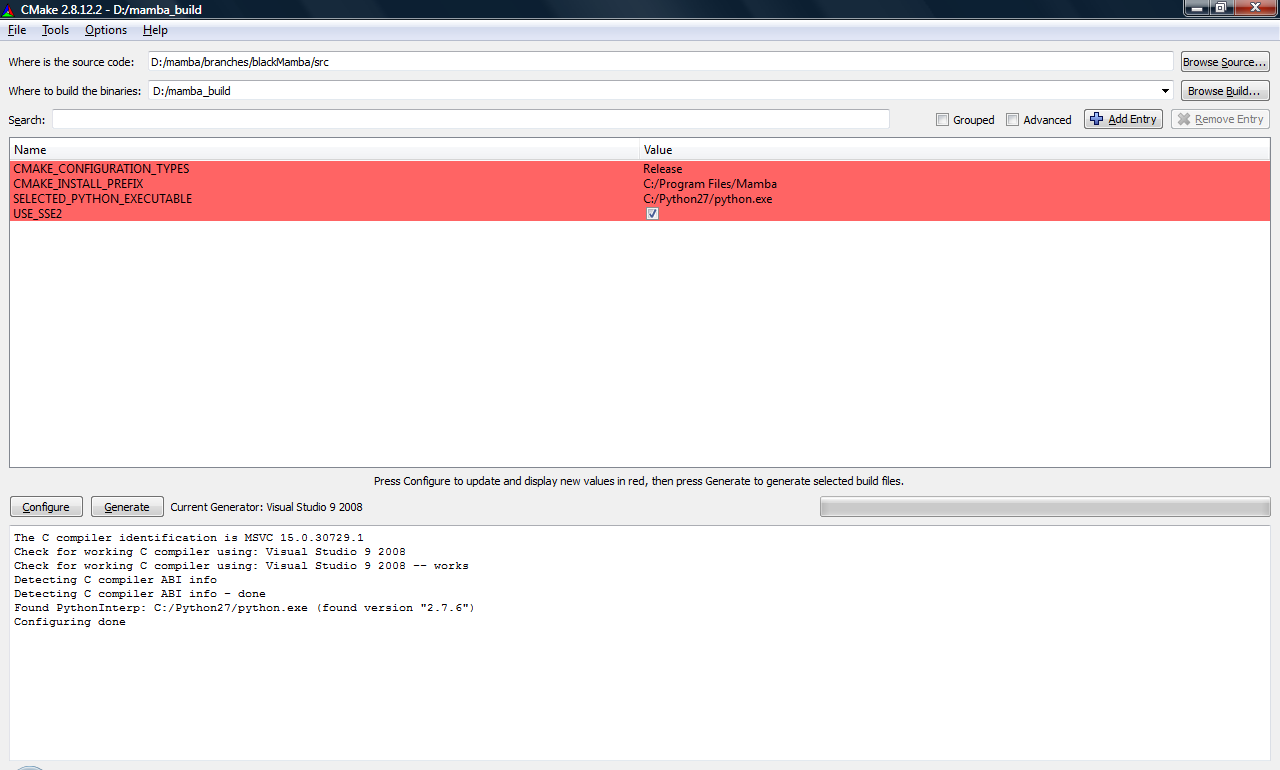
\includegraphics[scale=0.3]{images/cmake_win.png}
\caption{CMake configuration on Windows}
\label{fig:cmake_win}
\end{figure}

There are 4 configurable fields:
\begin{itemize}
\item \textbf{CMAKE\_CONFIGURATION\_TYPES}: Set this variable to "Release" to 
generate only the release configuration.
\item \textbf{CMAKE\_INSTALL\_PREFIX}: Ignore this option. It is a CMake 
mandatory that is not used by Mamba on Windows.
\item \textbf{SELECTED\_PYTHON\_EXECUTABLE}: Make sure this option points 
to your Python executable. In particular, if you have multiple Python 
installation on your computer you should verify that you are using the 
correct one.
\item \textbf{USE\_SSE2}: Only on 32-bit systems, allows you to enable (default)
or disable SSE2 support in Mamba. On 64-bit systems, SSE2 is always enabled.
\end{itemize}

Once you have set the configuration, you must press Configure again for it to
take effect. Then press "Generate". This should have created a Mamba.sln file
in the \textbf{mamba\_build} directory.

Open this file using Visual C++, you should see something similar to figure
\ref{fig:visualcpp}.

\begin{figure}
\centering
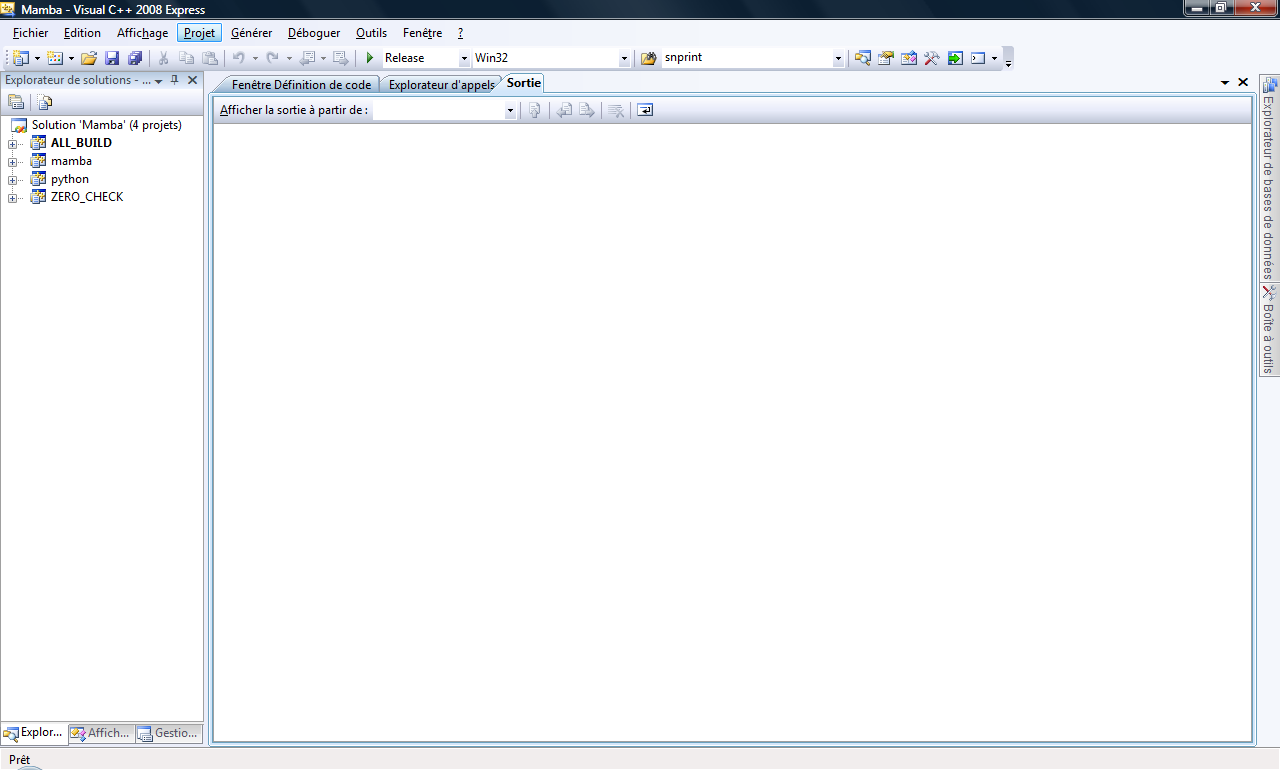
\includegraphics[scale=0.3]{images/visualcpp.png}
\caption{Visual C++ solution}
\label{fig:visualcpp}
\end{figure}

Open the menu \textit{"Generate"} and select \textit{"Generate ALL\_BUILD"}.
This should proceed with the compilation and the generation of the Python installer.

If everything went OK, you should find in the \textbf{mamba\_build} directory
the following files:
\begin{itemize}
\item the Python stand alone installer, Mamba Image-X.X.winYY-pyZ.Z.exe: in python/dist subdirectory.
\item C core library DLL (not needed for Python): mamba.dll, mamba.def, mamba.lib in lib/Release subdirectory
and include files in include subdirectory.
\end{itemize}

We strongly recommand you to verify the generated installer by installing it on
your computer and running the tests (see section \ref{cha:testing_mamba}).

\subsection{Linux}

As for Windows, you will have to create a directory where you will proceed with
the compilation and installation. Open a terminal and cd your way to this 
directory. Once there, type the following commands to compile and install on Linux:

\texttt{cmake -C path/to/Mamba.X.X/src}\\
\texttt{cmake -D CMAKE\_BUILD\_TYPE:STRING=Release -D CMAKE\_INSTALL\_PREFIX:STRING=/usr .}\\
\texttt{cmake -G "Unix Makefiles" .}\\
\texttt{make}\\
\texttt{su -c "make install python\_install"}

Of course you can use the CMake GUI to perform the first three operations.

In particular, if you want to compile Mamba for a different version of Python
the CMake GUI will give you access to the \textbf{SELECTED\_PYTHON\_EXECUTABLE}
variable to select the appropriate Python executable.

\subsection{Other platforms}

If you are not running one the afore-mentionned systems but still want to try
Mamba, you will need to find how to do it on your own. Currently, we have only access to
these kind of systems and thus cannot provide you with instructions on how to do
it with others. However, the basic requirements and instructions will likely apply.

By the way, if you have installed Mamba on another platform (successfully!), please
share your knowledge with others. We will be happy to insert your procedure in this
user manual (and give you credits...).

\pagebreak

\section{Using the library}
\label{cha:using_library}

This section explains how to use the library.

\subsection{Philosophy and implicit working of the library}

Before giving you details regarding how to fully grasp the library, we would
like to give you details regarding the way it implicitly works. This section aims
at presenting some aspects that will always be present in Mamba but likely not 
explained nor talked about.

When we talk about an \textit{empty} image or edge, this always means that pixels 
(inside or outside the image) take value 0. Thus an empty
image is an image where all the pixels are set to 0. On the opposite, the term 
\textit{filled} is always associated with the maximum possible value of a pixel (which
depends on the image depth).

All image pixels are stored with unsigned integers. This is true for binary,
greyscale and 32-bit images.

As a consequence of the coding rules applied to Mamba, functions image parameters
always begin with the input arguments and ends with the output arguments (This 
is a general rule and there may be some exceptions for particular functions).
Most of the time, images arguments are imIn when the image is an input and imOut
when it is the output of the function. When functions require arguments other than 
image arguments (scalar values, edge or grid settings, etc.), they are placed after 
the image arguments. Some images are both input and output and thus are named
imInOut.

When functions accept input and output images, you can safely use the same image
for both and you will obtain the expected result. If the function cannot 
guarantee this, it will return an error.

Regarding the mamba3D package, evrything was created to reuse as much as
possible the basic C operators from Mamba to perform the 3D computations so
as to avoid rewriting them (apart from hierarchical and labelling operators,
this was actually possible). Functions and classes are created with the same
"look and feel" as their counterpart in 2D.

These choices had consequences on the design of the package and thus on its
capacities. Overall we believe the possible downfall of that choices are
dimmed by the gains in terms of easiness of use, reuse of proven and robust
code and work versus objective ratio.

\subsection{A word for previous versions users}
\label{cha:change_mamba2}

Version 2 of Mamba introduced a lot of changes, made for performance and
easiness improvement, that \emph{will} break your scripts written for previous
versions (1.x). However, we believe this should not present too much of a
challenge to upgrade your scripts to the newest version.

The list of changes is quite long and we tried our best to not forget
anything important:
\begin{itemize}
\item All the Python sources (modules mamba.py, mambaDraw.py mambaExtra.py,
mambaDisplay.py and package mambaComposed) have been regrouped inside two packages
mamba and mambaDisplay. Functions and operators have also been reorganized
by families inside this package mainly for documentation purposes. This makes old
imports of Mamba incompatible. The mamba3D package, previously available as an
add-on, has been merged in the main library (both C and Python code). image3DMb 
now longer inherits from sequenceMb (other way around in Mamba 2).
\item The source reorganisation also impacts display with the creation of
the package mambaDisplay to contain both 2D and 3D displays. New displays were
added. Display methods in imageMb and image3DMb have been shortened (show,
hide, update instead of showDisplay ...). Palette and opacity methods were
removed from these classes. The 3D display methods were also strongly
modified by these changes.
\item Some operators were added (div), other were augmented or modified 
(label now supports 8-bit and 32-bit images and its default behavior regarding
label values has been changed, convert can be used with all image depths, close
and open operators were renamed closing and opening to avoid conflict with
Python standard functions, hitOrMiss now works directly with a
doubleStructuringElement object making binaryHMT useless, loadRaw methods were
homogenized for image3DMb and imageMb, copyBitPlane now supports 32-bit to
binary and reverse copies). C functions regarding neighbors (sup, inf, diff ...)
have been modified to gain performance. The corresponding Python functions are
also impacted. Support for hierarchical algorithms (watershed and build) on
32-bit images was added in C with removal of the specific Python functions
(namely watershedSegment32, basinSegment32, hierarBuild32 and hierarDualBuild32).
The operators are accessible through the standard functions (watershedSegment,
basinSegment, hierarBuild and hierarDualBuild).
\item Mamba is now compatible with Python 3. This may have impact on the
behavior of some functions (getDirections, for example, is based upon range
which does not have the same behavior in Python 3).
\item Mamba will no longer be supported on our part for Python 2.6. Mamba 2
needs ttk (themed Tk) for its display and the module is not natively available
in Python 2.6.
\item Mamba uses Pillow instead of PIL. You may have to update to Pillow if
you were a PIL user. Both library are normally equivalent in functionality
except for import mechanisms.
\item The C code is now compiled in a specific library (.dll or .so) with
its include files available separately making it possible to build applications
with the core functions of Mamba more easily. This has an impact on the
compilation process which now use CMake.
\item Mamba has support of Windows 64-bit thanks to available win64 packages
of Pillow.
\item Vectorisation in the C code was changed (see mambaApi\_vector.h).
\item The documentation was modified : directory containing doc in source renamed,
better use of doxygen to generate the C API doc, merge of the 2D and 3D doc,
separation of user manual and examples, change in the mamba style. Conversely,
some documents have been merged into the user manual.
\item The new version also means reorganisation of the source directory, of the
examples, of the tests.
\end{itemize}

The result of these changes is a faster and, we hope, more user-friendly
library.

\subsection{Contents of the library}

The Python Mamba library is composed of four packages:
\begin{itemize}
\item \textbf{mamba}, which is the main package of Mamba and contains all the operators
(from the most basic to quite advanced ones) to perform mathematical morphology
computations on 2D images.
\item  \textbf{mamba3D}, which contains the same operators (except some of them without
equivalent in a three dimensional context) working on 3D images.
\item  \textbf{mambaDisplay}, which contains all the code related to image displays for
both 2D and 3D.
\item  \textbf{mambaShell}, which is a container for functions and modules that are
needed to create and operate an appropriate shell for Mamba. In particular, it
contains demo presentations.
\end{itemize}

\subsection{Importing the packages}

To use Mamba, simply type in your Python console:

\lstset{language=Python}
\begin{lstlisting}
import mamba
import mamba3D
\end{lstlisting}

Both imports will give you access to the complete library (2D and 3D respectively).
You do not need to import mamba to use mamba3D or vice versa.

You can also use the following syntax:

\lstset{language=Python}
\begin{lstlisting}
from mamba import *
from mamba3D import *
\end{lstlisting}

There is no conflict between 2D and 3D functions (usually the later have the
same name postfixed 3D).

Other imports can be useful while working with mamba:

\lstset{language=Python}
\begin{lstlisting}
import mambaDisplay
import mambaDisplay.extra
\end{lstlisting}

They give you access to display management functions, palette functions and
extra displays.

\subsection{Grid and Edge}

Grid and edge are important notions in mathematical morphology. Let us explain
how they are handled in Mamba. 

\subsubsection{Edge}

The edge defines the status of all the pixels which are not in the image. Let us 
explain what this assertion means. Obviously, any image is made of a finite set 
of pixels. However, mathematical morphology operations, which are neighbourhood 
operations, need that the status of the neighbour points of the pixels which are at 
the edge of the image be defined, otherwise it would not be possible to define the 
transformation. This is the purpose of the edge attribute. The edge defines the 
virtual pixels which are outside the image. The edge (remember, it is the outside 
edge) can be set to \textbf{EMPTY} or \textbf{FILLED}. The \textbf{EMPTY} edge
is assuming that external world surrounding 
the image is made of virtual pixels at value 0 (the edge is set to 0) whereas 
the \textbf{FILLED} edge assumes an external world completely filled 
(the edge is set to the maximum possible value of a pixel according to the image 
depth). This notion applies to both 2D and 3D operators. See section \ref{cha:rules} for
further explanations on edge settings for 2D images.

Edge management for 3D images is a combination of two approaches as edges in a 3D image
are twofold. 3D images being made of a pile of 2D images, the edges parallel to the
\emph{z} axis are defined by the edges of the corresponding 2D images. These edges are
therefore virtual and their management is controlled by the \textit{edge} argument
(set to EMPTY or FILLED) of the 2D images. But two other edges must be defined. They correspond
to the floor and the ceiling (along the \emph{z} axis) of the 3D volume of data formed by a
3D image. Contrary to the 2D edges, these two ones are real and are built by adding two
supplementary 2D images set to 0 or to the maximum value (1, 255 or $2^{32} - 1$) depending
on the status (FILLED or EMPTY) of the 2D edge (figure \ref{fig:3D_edges}).

\begin{figure}
\centering
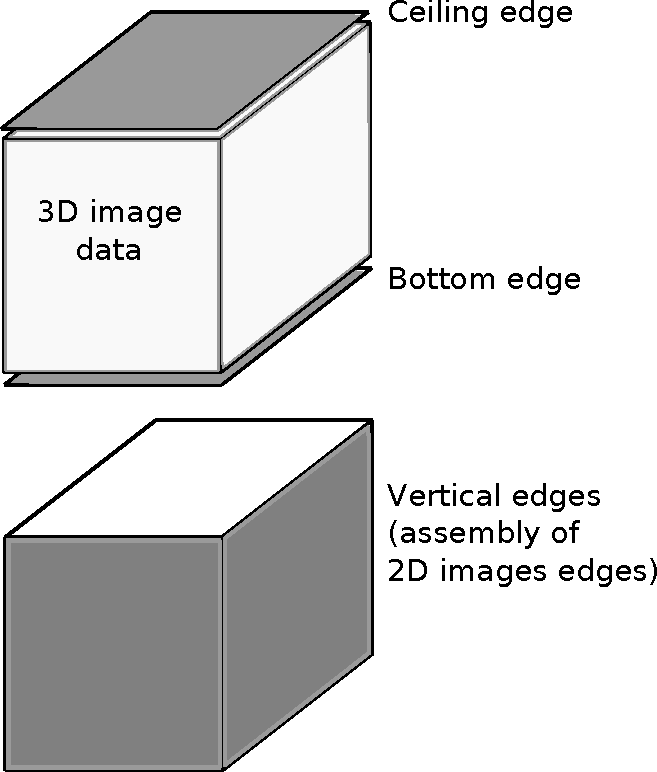
\includegraphics[scale=0.6]{figures/3D_edges.pdf}
\caption{Edges in a 3D image}
\label{fig:3D_edges}
\end{figure}

So, it is up to you, when defining operators where the edge status is relevant, to properly
manage this status. As an example, have a look on the definition of the erosions and dilations for 3D images.

\subsubsection{Grids 2D}
\label{cha:grid2D}

The grid defines the neighbourhood of each pixel in an image.

There are two possible grids in Mamba:

\begin{itemize}
\item \textbf{HEXAGONAL}: defines six neighbours for each pixel as can be seen in 
figure \ref{fig:hxgriddir}.

\begin{figure}
\centering
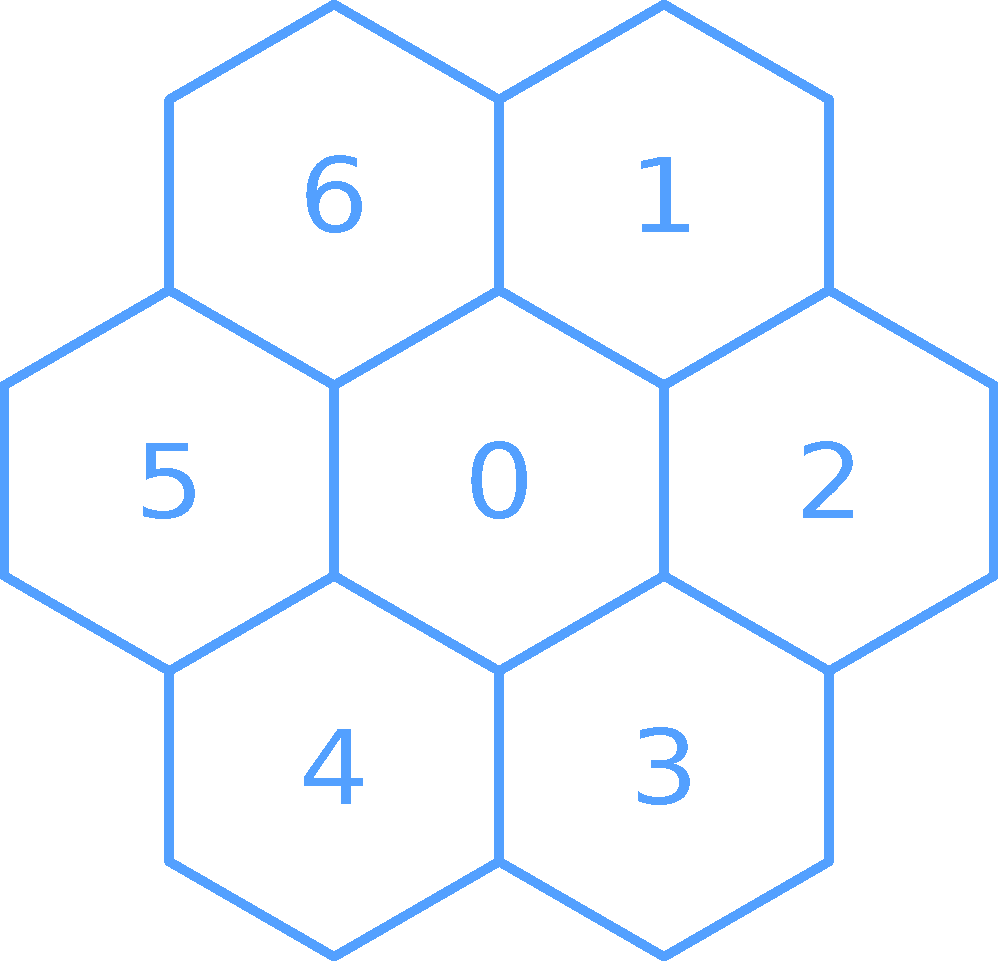
\includegraphics[width=0.2\textwidth]{figures/hexa_grid.pdf}
\caption{Hexagonal grid: representation and directions}
\label{fig:hxgriddir}
\end{figure}

\item \textbf{SQUARE}: defines the usual eight neighbours for each pixel as
in figure \ref{fig:sqgriddir}.

\begin{figure}
\centering
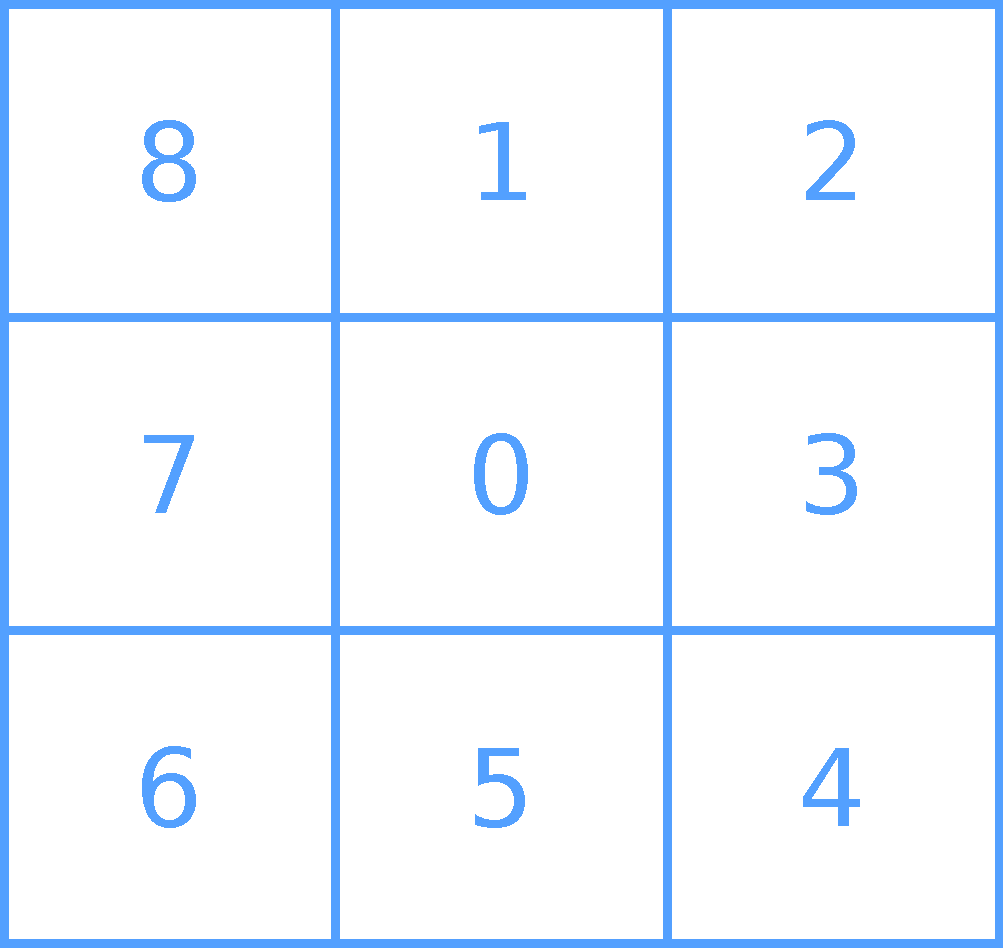
\includegraphics[width=0.2\textwidth]{figures/square_grid.pdf}
\caption{Square grid: representation and directions}
\label{fig:sqgriddir}
\end{figure}

\end{itemize}

2D grids are built-in grids. There is no way to modify them (that is to modify the neighborhood
relationships) under Python. These grids are straightforward and you can see the coding of the directions
defined on these grids in the documentation (Mamba Image Library Python Reference and Mamba API
Quick Reference manual), see section \ref{cha:other_docs}.

On the hexagonal grid, an image contains even lines (vertical coordinate multiple of 2) and odd lines. Even lines
are shifted to the left in relation to the odd lines, see figure \ref{fig:hex_grid}.
 
\begin{figure}
\centering
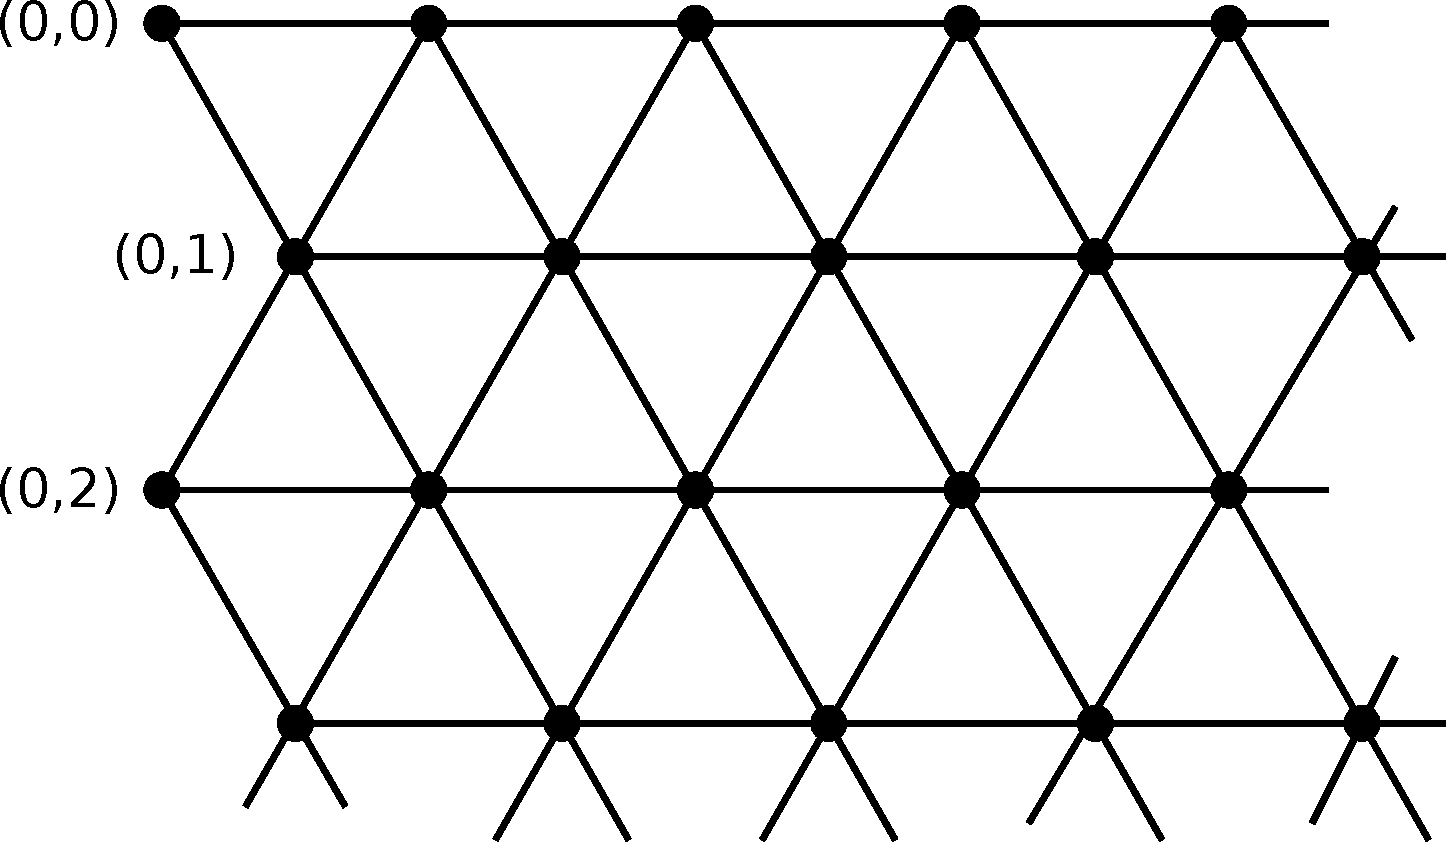
\includegraphics[scale=0.3]{figures/hex_grid.pdf}
\caption{Odd and even lines in the hexagonal grid}
\label{fig:hex_grid}
\end{figure}

As you will see later in this document, some functions need a direction or a 
neighbor as input. Figures \ref{fig:hxgriddir} and \ref{fig:sqgriddir} give you
the direction/neighbor encoding depending on the grid in use. The directions
are numbered from 0 to 6 or 8.

Some public operators are available with 2D grids (which are instances of a class \textbf{\_grid}). They are self
explanatory. See the documentation on the directions encoding for further details.

\subsubsection{Grids 3D}

There are three possible grids in 3D. They are a bit more
difficult to represent. Thus we will try to give you an overview
of what they look like. They also have some limitations that we think you
should be aware of.

As a foreword, we would like to explain how 3D grids are built.
Instead of the 2D ones which are defined for low-level C operators, 3D
grids are very high level complex structures. They are built using 2D grids and
a mix of programmation magic. Some operators were rewritten in low-level C
functions working on 3D images because their 2D counterpart could not be adapted
to a 3D structure (e.g. hierarchical queues operators). As they work using the
grid, we defined some grids in low-level C but not all of them (too much work).
So some operators may not work with the grid you selected. Be warned !

A 3D grid is defined by providing two settings:

\begin{itemize}
\item The 2D grid (hexagonal or square) which is used with the 2D image sections of the 3D image.
\item The way these 2D images are stacked, this stacking defining the neighborhood relationships in the 3D grid.
\end{itemize}

\tipBox{
Grids in Mamba3D are strongly influenced by crystallography. For example,
the face centered cubic grid is describing the way carbon atoms are 
crystallized to form diamonds and the centered cubic one (also named body centered
cubic) is a structure by which iron atoms organise themselves. Of course, there
is a lot of other structures in crystals that are not represented in Mamba3D.
}

Three grids are defined in Mamba3D (they are represented by means of top views and perspective views,
with the coreesponding directions/neighbors numbers):

\begin{itemize}
\item \textbf{CUBIC (C)}: The very basic cubic grid, built by stacking square
grids one on the other. See figures \ref{fig:cubic_grid} and \ref{fig:cubic_grid_3D}.
\item \textbf{FACE\_CENTER\_CUBIC (FCC)}: A face centered cubic grid. It is in fact
built by stacking hexagonal grids one on the other with a slight shift. See
figures \ref{fig:fcc_grid} and \ref{fig:fcc_grid_3D}.
\item \textbf{CENTER\_CUBIC (CC)}: Also known as body centered cubic, this grid is
built by stacking square grids with a half shift in the two directions. See
figures \ref{fig:ccubic_grid} and \ref{fig:ccubic_grid_3D}. This grid is not
supported by low-level C operators.
\end{itemize}

These grids are instances of a \textbf{\_grid3D} class. Each grid comes with various
methods to handle it. Some of them are similar to the operators provided with 2D grids.
However, some others are specific and are more complex.

For each 3D grid, The 2D grid on which it is based is given by the method \textbf{get2DGrid}.

In addition, three specific methods come with 3D grids: \textbf{getEncodedDirs}, \textbf{convertFromDir}
and \textbf{getShiftDirsList}.

\begin{itemize}
\item \textbf{getEncodedDirs} is mainly used with 3D structuring elements. It allows to
decompose any elementary 3D structuring element (defined by a list of directions) into
three 2D structuring elements corresponding to the three sections of the initial 3D structuring
element, see section \ref{cha:structelem} for further explanations.
\item \textbf{convertFromDir} requires two parameters: a 3D direction and the \emph{z} coordinate
of the pixel. It returns a tuple containing the section (-1 if below, 0 if current and 1 if above)
and the 2D direction in this section corresponding to the 3D direction and to the \emph{z} position of the
pixel. This method is quite useful to increase the computation speed of some 3D operators like shiftings as it
provides directly the \emph{z} offset and the corresponding horizontal direction (at least for the cubic
grid - for the others, it is a bit more complex) of this shifting.
\item \textbf{getShiftDirsList} is a more complex method mainly used in the 3D shift operator (shift3D) and
in the infFarNeighbor3D and supFarNeighbor3D operators. This method requires three parameters: a 3D
direction \emph{d}, the amplitude (size) \emph{amp} of the shift applied in this direction and the
z coordinate of the pixel (or the section) which will be shifted, \emph{zindex}. It returns
a list (of variable length) containing tuples (dh, amph, grid2D), each one providing the horizontal
direction \emph{dh}, the horizontal amplitude \emph{amph} of the corresponding horizontal shift which
will be applied on each section. \emph{grid2D} indicates the 2D grid on which this 2D shift will be performed.
\end{itemize}

These methods will be explicited below for the different grids.

\paragraph{Cubic grid\\}

\begin{figure}
\centering
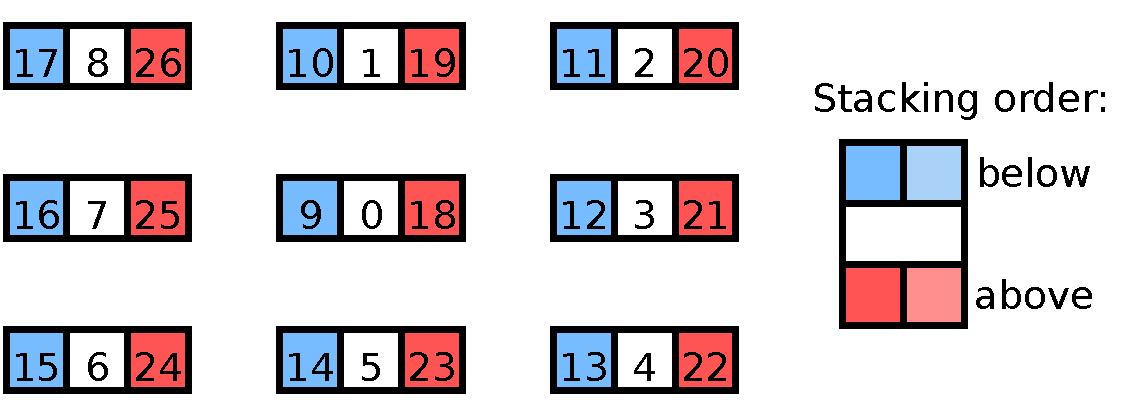
\includegraphics[width=0.55\textwidth]{figures/cubic_grid.pdf}
\caption{Cubic grid, top view}
\label{fig:cubic_grid}
\end{figure}

\begin{figure}
\centering
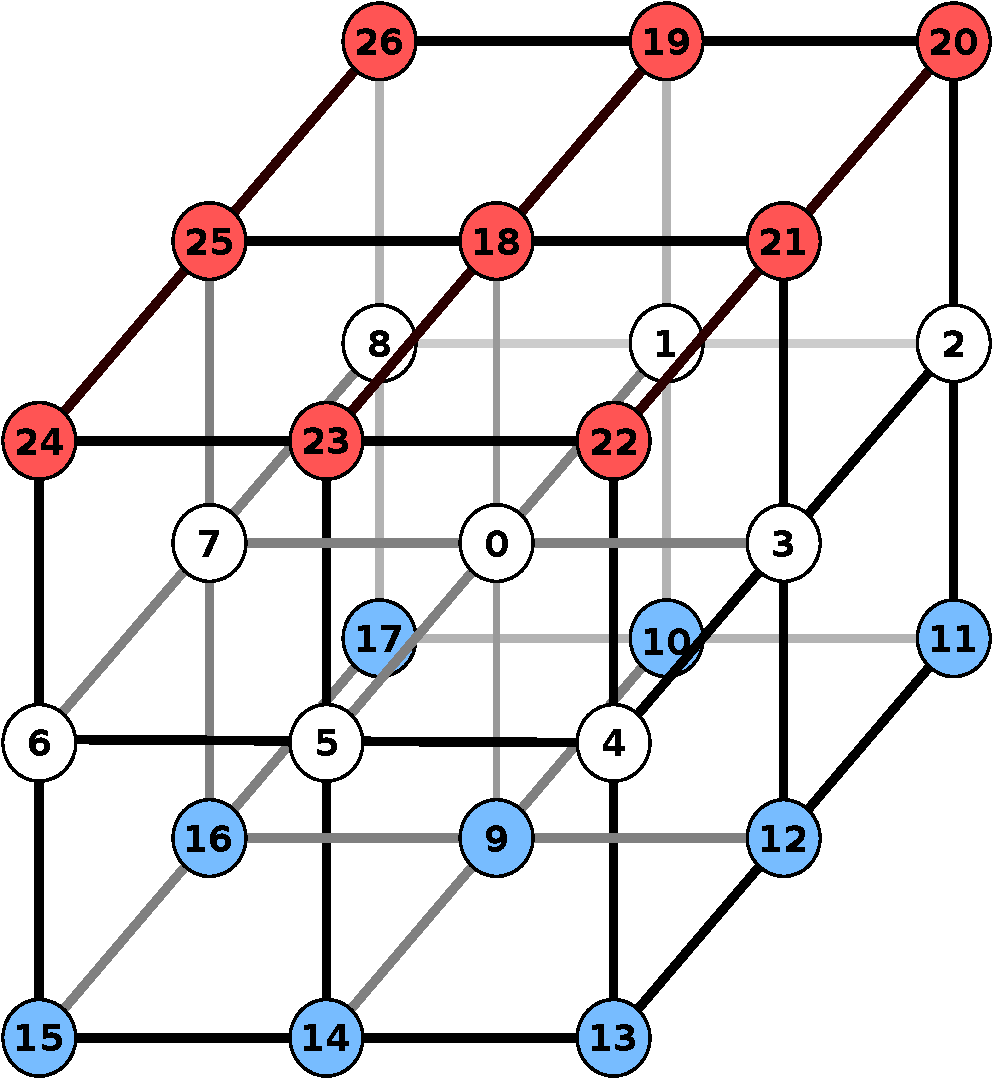
\includegraphics[width=0.5\textwidth]{figures/Cubic_grid_3D.pdf}
\caption{Cubic grid, perspective view}
\label{fig:cubic_grid_3D}
\end{figure}


This grid (named CUBIC) is made by stacking 2D images defined with a square grid (figures \ref{fig:cubic_grid} and \ref{fig:cubic_grid_3D}).

\lstset{language=Python}
\begin{lstlisting}
>>> CUBIC.get2DGrid()
SQUARE
\end{lstlisting}

Each pixel of the cubic grid is surrounded by 26 neighbors, associated to 26 directions scattered among the section containing the
central pixel (8 directions) and the two sections below and above it (9 directions each).

\lstset{language=Python}
\begin{lstlisting}
>>> CUBIC.convertFromDir(12, 5)
(-1, 3)
\end{lstlisting}

The direction 12 in the cubic grid corresponds to the direction 3 in the section below section 5.

Note that, for the cubic grid, the result is the same whatever \emph{z} because all the 2D images are stacked without shifting. It is
not the case for the other grids (see below).

\lstset{language=Python}
\begin{lstlisting}
>>> CUBIC.getShiftDirsList(11, 23, 49)
[(2, 23, SQUARE)]
\end{lstlisting}
 
A shift of size 23 in direction 11 on the cubic grid for the image section 49 corresponds to an horizontal shift of size 23 in
direction 2. So, a shift of section 49 is performed by an horizontal shift of size 23 in direction 2. The shifted 2D image is then stored
in section 26 (49 - 23, it is a downwards shift) of the output 3D image. In the case of the cubic grid, the operation is straightforward.
But it is not the case with the other 3D grids. It may also seem strange to
indicate which 2D grid is used to perform the horizontal shift. Here again, on the cubic grid, this information is redundant. But
we shall see, for the FCC grid, that this information is necessary to cope with edge effects.
  
\paragraph{Centered cubic grid\\}

Here again, this grid (named CENTER\_CUBIC) is defined by stacking 2D images defined with a square grid. But the odd sections
are shifted compared to the even sections just below so that the pixels be placed in the middle of the 2x2 squares of the below
section, hence the name "centered cubic (figures \ref{fig:ccubic_grid} and \ref{fig:ccubic_grid_3D}). Therefore, this grid is
made of an assembly of two shifted square grids which is repeated all along the \emph{z} axis.

\begin{figure}
\centering
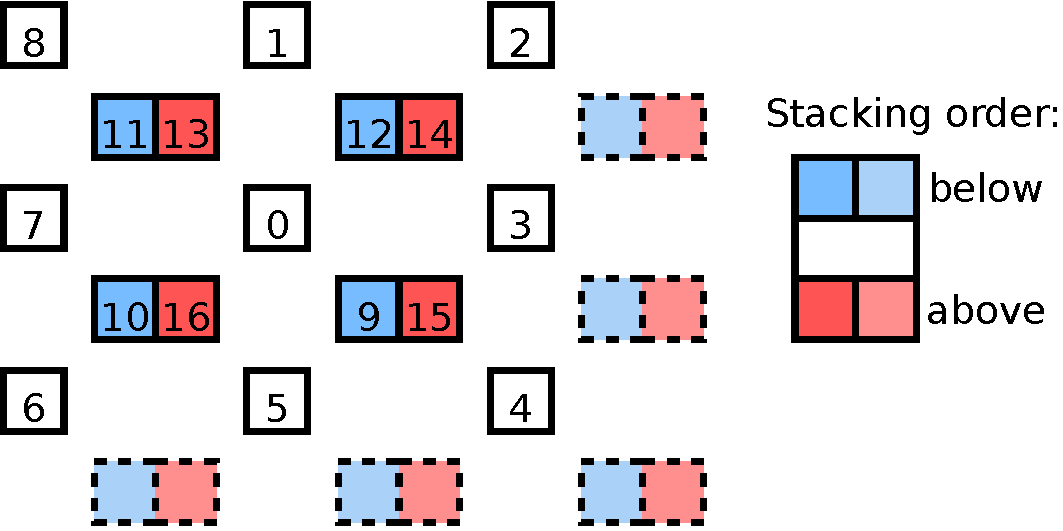
\includegraphics[width=0.55\textwidth]{figures/ccubic_grid.pdf}
\caption{Centered cubic grid, top view}
\label{fig:ccubic_grid}
\end{figure}

\begin{figure}
\centering
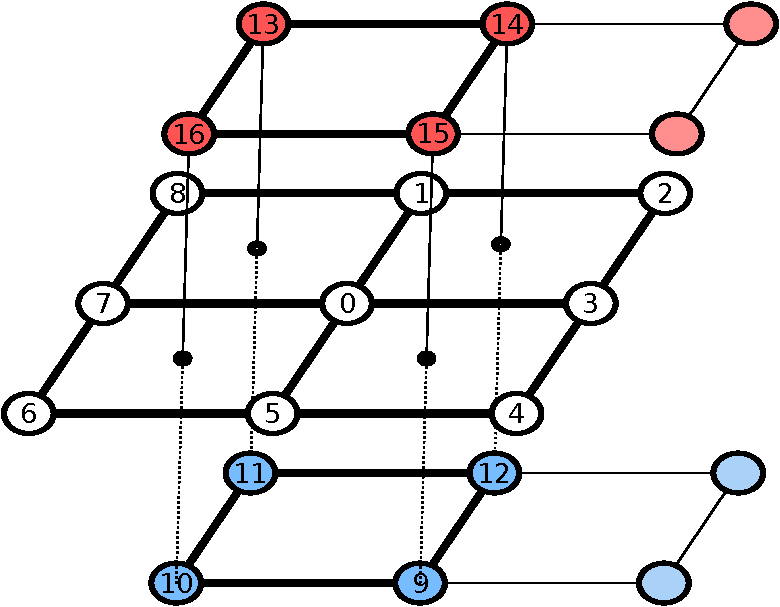
\includegraphics[width=0.5\textwidth]{figures/Ccubic_grid_3D.pdf}
\caption{Centered cubic grid, perspective view}
\label{fig:ccubic_grid_3D}
\end{figure}

Figure \ref{fig:CC_grid} shows the relative arrangement of the odd and even planes.

\begin{figure}
\centering
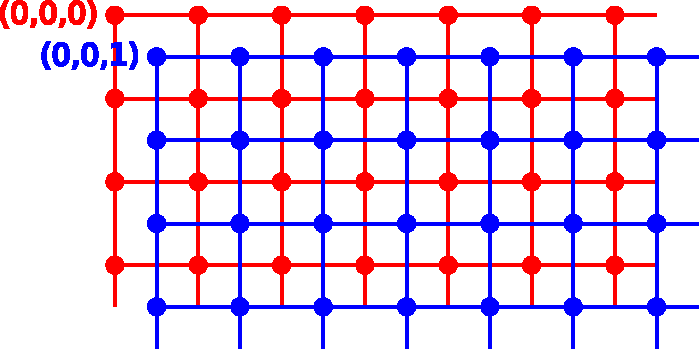
\includegraphics[scale=0.8]{figures/CC_grid.pdf}
\caption{Planes arrangement in the centered cubic grid}
\label{fig:CC_grid}
\end{figure}

Therefore, the \textbf{convertFromDir} operator returns a result which depends on the parity of the \emph{z} coordinate of the pixels:

\lstset{language=Python}
\begin{lstlisting}
>>> CENTER_CUBIC.convertFromdir(15, 0)
(1, 0)
>>> CENTER_CUBIC.convertFromdir(15, 1)
(1, 4)
\end{lstlisting}

Calculating the horizontal offsets in shifting operations is then more complicated as it depends of the relative parities
of the starting and ending planes.

On this grid, \textbf{getShiftDirsList} returns a list of horizontal shifting directions and amplitudes which strongly depend
on the 3D amplitudes and on the parity of the z index. We have for instance:

\lstset{language=Python}
\begin{lstlisting}
>>> CENTER_CUBIC.getShiftDirsList(14, 10, 4)
[(1, 5, SQUARE), (3, 5, SQUARE)]
>>> CENTER_CUBIC.getShiftDirsList(14, 11, 5)
[(1, 5, SQUARE), (3, 6, SQUARE)]
>>> CENTER_CUBIC.getShiftDirsList(14, 11, 6)
[(1, 6, SQUARE), (3, 5, SQUARE)]
\end{lstlisting}

Some directions only need one shift:

\lstset{language=Python}
\begin{lstlisting}
>>> CENTER_CUBIC.getShiftDirsList(9, 11, 4)
[(4, 5, SQUARE)]
\end{lstlisting}

\paragraph{Face centered cubic grid\\}

The face centered cubic grid (named FACE\_CENTER\_CUBIC) is the most complex grid defined in Mamba3D. The 2D base grid is hexagonal
and the 3D grid is obtained by piling and shifting these 2D hexagonal grids (figures \ref{fig:fcc_grid} and \ref{fig:fcc_grid_3D}).

\begin{figure}
\centering
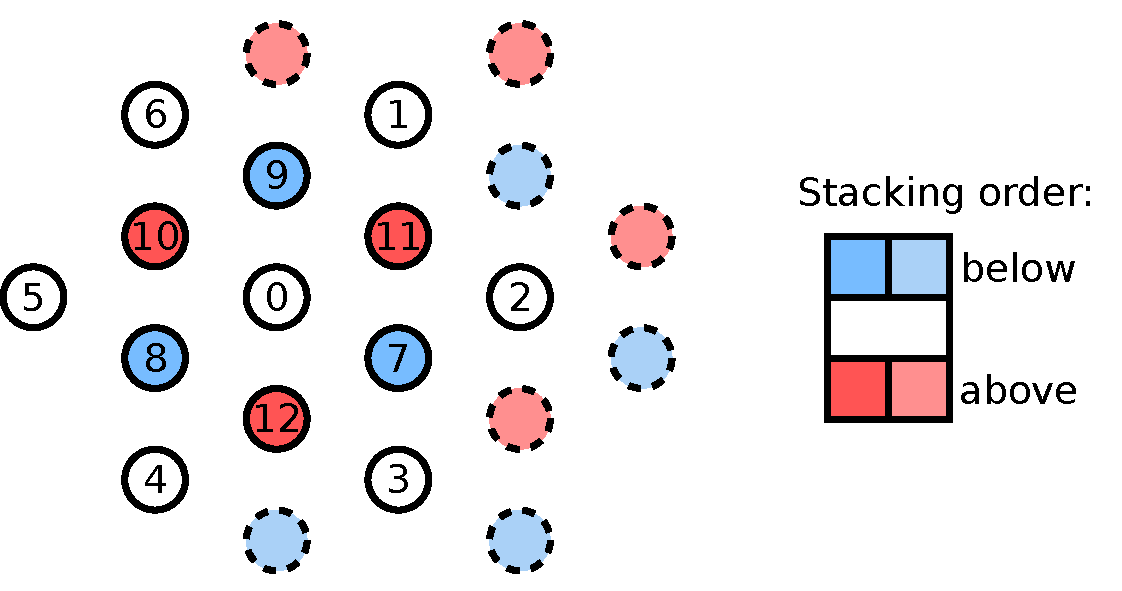
\includegraphics[width=0.55\textwidth]{figures/fcc_grid.pdf}
\caption{Face centered cubic grid, top view}
\label{fig:fcc_grid}
\end{figure}

\begin{figure}
\centering
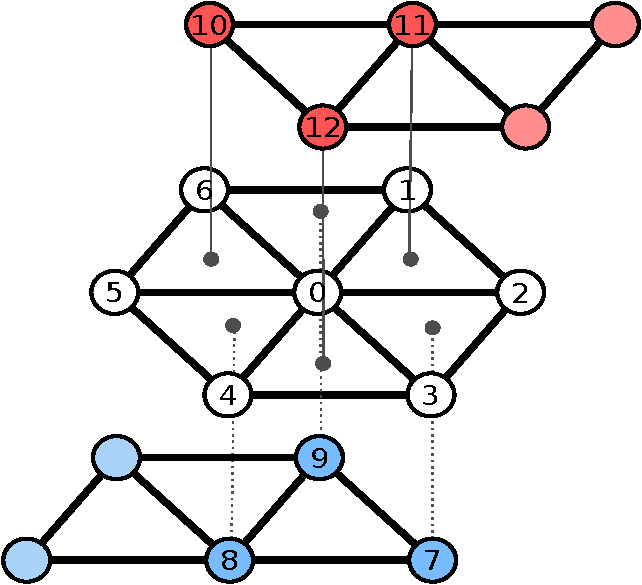
\includegraphics[width=0.5\textwidth]{figures/Fccubic_grid_3D.pdf}
\caption{Face centered cubic grid, perspective view}
\label{fig:fcc_grid_3D}
\end{figure}

In this case, three 2D hexagonal grids are used and shifted according to the scheme given in figure \ref{fig:FCC_grid_piling}.
Then, this configuration is repeated along the \emph{z} axis.

\begin{figure}
\centering
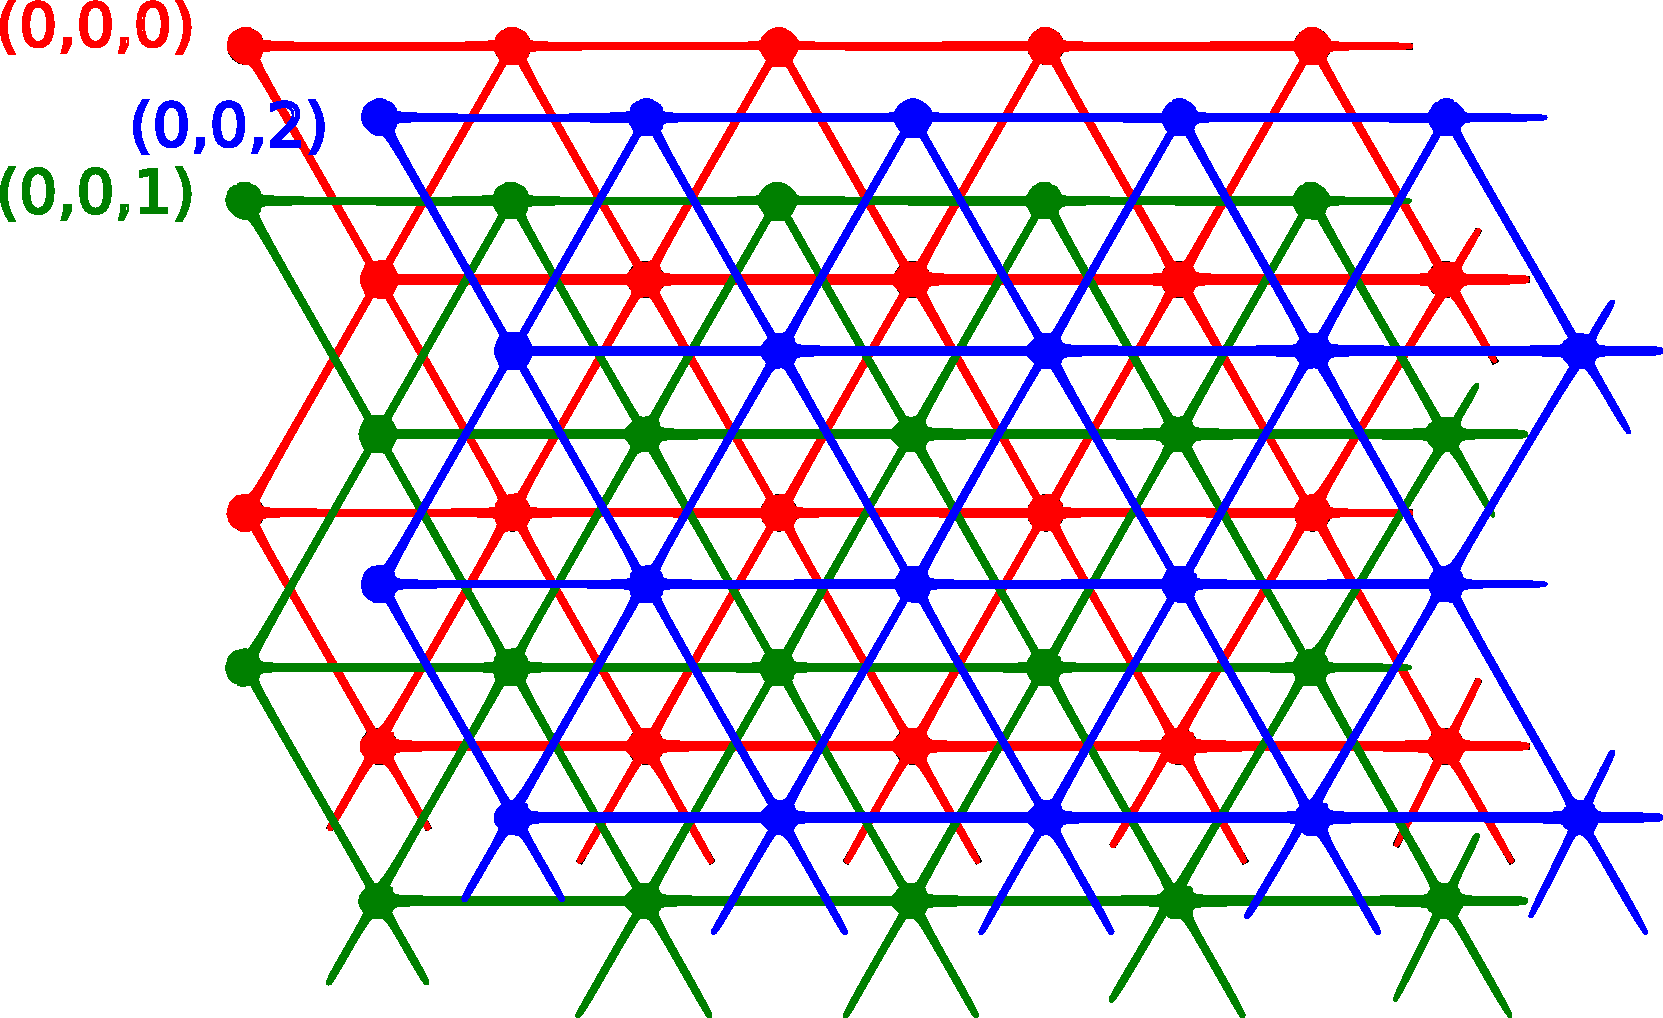
\includegraphics[scale=0.5]{figures/FCC_grid_piling.pdf}
\caption{Planes arrangement in the face centered cubic grid}
\label{fig:FCC_grid_piling}
\end{figure}

You can notice on figure \ref{fig:fcc_grid_3D}
that the triangles drawn by below directions (blue) and above directions (red)
do not point the same way. Stacking and shifting 3 planes (instead of 2 as for
the centered cubic grid) allows to define symmetrical structuring elements (cuboctahedrons).
Shifting only two planes would produce another grid structure named \textit{hexagonal
closed packed} structure. Unfortunately, the structuring elements defined on this grid
are not symmetrical (we have in particular anticuboctahedrons).

The \textbf{convertFromDir} operator provides different results according to the
congruence modulo 3 of the \emph{z} coordinate with the values 0, 1 and 2:

\lstset{language=Python}
\begin{lstlisting}
>>> FACE_CENTER_CUBIC.convertFromdir(10, 0)
(1, 6)
>>> FACE_CENTER_CUBIC.convertFromdir(10, 1)
(1, 5)
>>> FACE_CENTER_CUBIC.convertFromDir(10, 2)
(1, 0)
\end{lstlisting}

On this FCC grid, \textbf{getShiftDirsList} returns horizontal directions on the hexagonal grid corresponding to 3D directions. For instance:

\lstset{language=Python}
\begin{lstlisting}
>>> FACE_CENTER_CUBIC.getShiftDirsList(10, 11, 4)
[(6, 3, HEXAGONAL), (5, 4, HEXAGONAL)]
\end{lstlisting}

However, in directions 9 and 12, one direction is defined on the square grid:

\lstset{language=Python}
\begin{lstlisting}
>>> FACE_CENTER_CUBIC.getShiftDirsList(9, 11, 5)
[(1, 6, SQUARE), (1, 1, HEXAGONAL)]
\end{lstlisting}

This trick allows to avoid edge effects which would happen if the hexagonal grid was used. Indeed, in this case, the first shift would
likely send a shifted pixel close to the edge outside of the image window with no possibility to recover it with the second shift.
 
\subsubsection{More on 2D and 3D grids}

As it is, we could have added a lot more grids in Mamba3D. For example,
we could have built a grid stacking without any shifted hexagonal grids.
We chose not to do it, but it does not mean you can't, although we doubt very
much you find such grids useful. In this event, we encourage you to look
at section \ref{cha:create_grid3D}.

Be aware that the grid is never an image attribute, but a structuring element 
attribute. A structuring element is always defined on a given grid. Therefore, 
when performing a transformation with a given structuring element, the corresponding 
grid will be used with the image. Changing the grid of a 2D image can be seen as a 
simple shift of the even lines of the image versus the odd ones so that the pixels 
belonging to an even line are between the pixels of the following odd line. The even 
lines are shifted to the right compared to the odd ones (the first line is numbered 0, 
it is therefore an even one). See section \ref{cha:grid2D} for further details.

By default, when it is launched, Mamba uses the \textbf{HEXAGONAL} grid (through 
the DEFAULT\_GRID variable). Mamba3D uses the \textbf{FACE\_CENTER\_CUBIC} grid
(through the DEFAULT\_GRID3D variable)  Each function requiring a grid
configuration as a parameter is given DEFAULT\_GRID(3D) by default. When an
edge status is needed, the default value is selected depending on the operator
in use. The edge, as the grid, is not an image attribute.

There are different ways to change the grid. You can use the setDefaultGrid 
(setDefaultGrid3D for Mamba3D) function:

\lstset{language=Python}
\begin{lstlisting}

# Changes the default grid (DEFAULT_GRID) to HEXAGONAL
setDefaultGrid(HEXAGONAL)

# Changes the default grid (DEFAULT_GRID) to SQUARE
setDefaultGrid(SQUARE)
\end{lstlisting}

You can change the grid used when calling the operator.

You can get a list of all the available directions of a grid
by calling the function getDirections (getDirections3D for Mamba3D).

\lstset{language=Python}
\begin{lstlisting}
# Returns a list of all the available directions for the default grid
directions = getDirections()
# Returns a list of all the available directions for the SQUARE grid
directions = getDirections(SQUARE)
# Returns a list of all the available directions for the HEXAGONAL grid
directions = getDirections(HEXAGONAL)
\end{lstlisting}

There are other utilities functions that are provided by Mamba and Mamba3D to
handle  directions/neighbors. Refer to the Python API reference manual.

\subsection{Creating and manipulating images}
\label{cha:create_im}

\subsubsection{2D images}

To handle images, a Python class named \textbf{imageMb} has been created. This class will allow
you to create, load, save and perform standard operations on your images.

An image is basically an array of pixels. Each pixel is referred by its coordinates (x,y), see
figure \ref{fig:image_coord}. Each pixel can take a 1-bit (binary), 8-bit (greyscale) or 32-bit value.
This parameter is called \textit{depth} of the image. If you want to process 16-bit images, you will have to
load them in a 32-bit Mamba image (which is actually not at all a problem).

\textit{Width} w and \textit{heighth} are the two other parameters (attributes) of an image. \textit{width} is the number of
pixels per line in the horizontal direction, \textit{height} the number of lines (or the number of pixels in
the vertical direction), see figure \ref{fig:image_coord}.

\begin{figure}
\centering
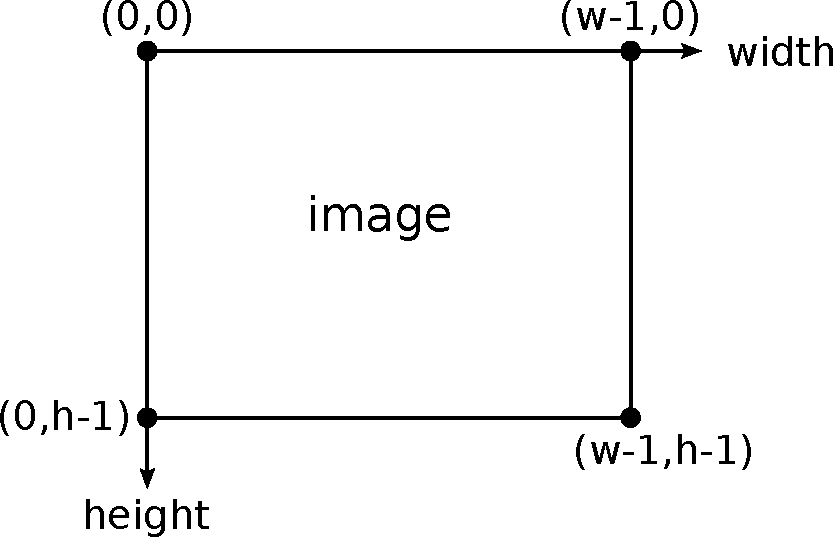
\includegraphics[scale=0.7]{figures/image_coord.pdf}
\caption{Image pixels coordinates}
\label{fig:image_coord}
\end{figure}

The imageMb constructor offers a wide range of possibilities to create an image. 
Here is the list of all these possibilities:

\begin{itemize}
\item \texttt{\textbf{imageMb()}}, without arguments, will create an empty 
256x256 greyscale image.
\item \texttt{\textbf{imageMb(im)}} will create an image using the same size 
and depth than 'im'.
\item \texttt{\textbf{imageMb(depth)}} will create an image with the desired
'depth' (1, 8 or 32).
\item \texttt{\textbf{imageMb(path)}} will load the image located in 'path'.
\item \texttt{\textbf{imageMb(im, depth)}} will create an image using the same 
size than 'im' and the specified 'depth'.
\item \texttt{\textbf{imageMb(path, depth)}} will load the image located in 
'path' and convert it to the specified 'depth'.
\item \texttt{\textbf{imageMb(width, height)}} will create an image with size 
'width'x'height'.
\item \texttt{\textbf{imageMb(width, height, depth)}} will create an image with
size 'width'x'height' and 'depth'.
\end{itemize}

When not specified, the width and height of the image will be set to 
256x256. The default depth is 8 (greyscale).

2D images can be defined with any positive w and h values. However, Mamba
works only with images that have a width multiple of
64 and a height multiple of 2. It means that if you requested the creation of
an image of size 747x621, Mamba will actually create an image of size 768x622. 
The actual image is always larger than or equal to the defined size.

\lstset{language=Python}
\begin{lstlisting}
>>> im = imageMb(747, 621)
>>> im.getSize()
(768, 622) 
\end{lstlisting}

Two factors explain this particularity:

\begin{itemize}
\item In order to increase the processing speed, pixel values are stored in words and these
words may be 64 bits long if your OS allows it. By this means, 64 pixels of a binary image
are stored in a single word and then processed in parallel. The result is a dramatic increase
of the computation speed. So, if the horizontal size of the image is not multiple of 64, this could
deeply deteriorate the performance, as each end of line should be processed differently. 
\item Similarly, if the height is not even, a supplementary line is added to the image. The
reason is that the image can be processed on an hexagonal grid (see section \ref{cha:grid2D}). In this case and to
avoid again to increase the complexity of the operators, the number of even lines must be equal to
the number of odd ones.
\end{itemize}

The pixels added to the image are set to 0. This procedure is called padding. Padding may seem confusing
because it adds strips of black pixels on the right and bottom of the image. Therefore, processing such an
image leads to unwanted edge effects. The erosions for instance increase the size of the black strips
but many other operators are also concerned.

A better solution consists in cropping the image, that is cutting it in order to let it fit to the image size.
However, padding has been preferred to cropping because it allows the user not to lose any pixel of the image
and to choose at the end the part of it which will be discarded by cropping.

Nevertheless, cropping can be performed by two means:

\begin{itemize}
\item \textbf{cropCopy} can be used to extract from the padded image the part which interests you. Note that
\textbf{cropCopy} does not clear the destination image, it simply replace the cropped part (see the Mamba
Image Examples manual (section \ref{cha:other_docs}).
\item The size of the destination image can also be set before loading the image file:

\lstset{language=Python}
\begin{lstlisting}
>>> im = imageMb(256, 256)
>>> im.load("myimage.png")
\end{lstlisting}

"myimage.png" is a (300x300) image stored in the Python working directory. This solution however does not allow you
to choose the part of the image which will be loaded: it is always the upper left part.
\end{itemize}

\tipBox{
Mamba allows you to create images with different sizes but not to perform
computations between them. If you want to do so, you will have to use the
cropCopy() function to extract the part of the images you want to match.
}
There is also a size limitation when you define images. This limitation is given by
the number of pixels in the image which must be lower than or equal to $2^{32}$.
This is a really huge value which allows you to define 65536x65536 images for instance.
A 200000x10000 image is also allowed (number of pixels lower than the limit).
Note however that, in practice, the real allowed maximum size is smaller as you would
need a fairly huge amount of memory to handle these images in Mamba. So, be sure
that your memory space is sufficient if you intend to use big images.

\subsubsection{3D images}

The basic data model used in Mamba3D is the \textbf{image3DMb} image class. This class is the
complete equivalent to the imageMb class for 3D images and it inherits its attributes and methods.
New attributes and methods are defined to deal with these images.

You should know that this class is actually a stack of standard Mamba images
(imageMb object) with all the same size and depth. The dimension of a 3D image
is thus given by the size of the Mamba images inside the stack and by its
length. Contrary to the two other dimensions, there is no restriction
on the value of \textit{length}.. This choice may seem strange because it differentiates one direction
(supposedly z-axis) in the data structure from the other two (x-axis and
y-axis) but it was dictated by the need to reuse as much as possible the 
basic C functions of Mamba which work with the imageMb low-level structure.

A 3D image is in fact a list of 2D images. Therefore, each 2D image at position \emph{i}
(the indexing starts at 0) composing the 3D image im3D can
be accessed by:

\lstset{language=Python}
\begin{lstlisting}
im3D[i]
\end{lstlisting}

\begin{figure}
\centering
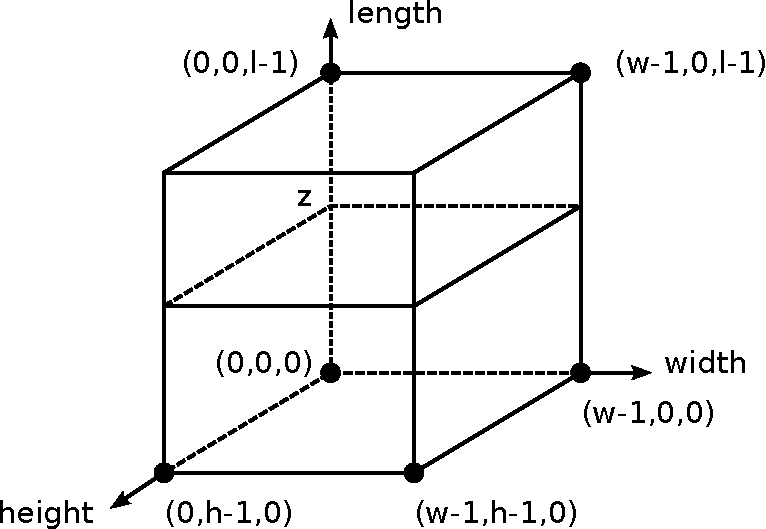
\includegraphics[scale=0.8]{figures/image3D_coord.pdf}
\caption{Image 3D pixels coordinates}
\label{fig:image3D_coord}
\end{figure}

Figure \ref{fig:image3D_coord} shows the coordinates arrangement of a 3D Mamba image. The length of the pile of 2D images (the third
dimension of the 3D image) corresponds to the length of the im3D list:

\lstset{language=Python}
\begin{lstlisting}
imLength = len(im3D)
\end{lstlisting}

There is a wide range of possibilities to create a 3D image object :
\begin{itemize}
\item \texttt{\textbf{image3DMb()}} : without arguments will create an empty
greyscale 3D image (by default its size is 256x256x256).
\item \texttt{\textbf{image3DMb(im3D)}} : will create a 3D image using the
same width, height, length and depth than 3D image 'im3D'.
\item \texttt{\textbf{image3DMb(im)}} : will create a 3D image using the same
width, height and depth than 2D image 'im' (a imageMb object). Its
length will be defaulted to 256.
\item \texttt{\textbf{image3DMb(depth)}} : will create a 3D image with the
desired 'depth' (1, 8 or 32) and default size (256x256x256).
\item \texttt{\textbf{image3DMb(path)}} : will load the image sequence located
in 'path', see the load method.
\item \texttt{\textbf{image3DMb(im3D, depth)}} : will create a 3D image using
the same size than 3D image 'im3D' and the specified 'depth'.
\item \texttt{\textbf{image3DMb(im, length)}} : will create a sequence using
the same width, height and depth than 2D image 'im' (a imageMb object). Its
length will be the specified 'length'.
\item \texttt{\textbf{image3DMb(path, depth)}} : will load the image sequence
located in 'path' and convert it to the specified 'depth'.
\item \texttt{\textbf{image3DMb(width, height, length)}} : will create a 
greyscale 3D image with 'width', 'height' and 'length'.
\item \texttt{\textbf{image3DMb(width, height, length, depth)}} : will create
a 3D image with the given parameters.
\end{itemize}

In the new release of Mamba (2.x), the \textbf{sequenceMb} class is simply an alias of the \textbf{image3DMb} class.
Indeed, a sequence is simply a list of 2D images. It can be considered as a special case of 3D image where
the third dimension is time.

\subsubsection{Saving and loading images}

\paragraph{2D images\\}

Upon creation of after you created an image you can load it with the data
contained inside a file. Loading an image, either at construction or
with the load method, makes use of the Pillow library. Any image format supported
by this library will then be supported by Mamba.

You can proceed like this:

\lstset{language=Python}
\begin{lstlisting}
# Loading the content of test.png in image im1
im1.load('test.png')
# Creating an image with the content of test.png loaded at start
im2 = imageMb('test.png')
\end{lstlisting}

Loading an image after the creation will not change the size of the original 
image to adapt it to the loaded image. The loaded image is padded/cropped to fit
the original size. Whereas, when the image is loaded in the constructor, its size
is used as an information for the imageMb size.

Pillow images came with a mode property that depends on the type of image.
Here are the rules applied when converting from Pillow to Mamba:

\begin{center}
\begin{tabular}{|c|c|}
  \hline
  Pillow mode & Mamba depth \\
  \hline
  "1" & 8\\
  "L" & 8\\
  "P" & 8\\
  "RGB" & 8 (using rgbfilter)\\
  "RGBA" & 8 (using rgbfilter)\\
  "CMYK" & 8 (using rgbfilter)\\
  "I" & 32\\ 
  "F" & 32\\
  \hline
\end{tabular}
\end{center}

For RGB, RGBA and CMKY formats, you can specify the RGB filter that will be
used to convert color image into greyscale image by adding the
rgbfilter=<your\_filter> to the argument of the constructor (see Pillow
documentation for examples of filters).

With the load method, when the loaded Mamba image depth is not the depth
of the destination image, it is converted to the correct depth.

Once you have created an image and performed some operations on it, you may want 
to save it into a file. The imageMb class provides the method save() to do so:

\lstset{language=Python}
\begin{lstlisting}
# Saving the content of im1 image in test.png
im1.save('test.png')
\end{lstlisting}

The method uses Pillow functions to save the image. Thus the format (bmp, gif, 
jpeg, ...) is automatically deduced from the extension used.

As for the load method, the conversion from a Mamba image to a Pillow image
applies the following rules:

\begin{center}
\begin{tabular}{|c|c|}
  \hline
  Mamba depth & Pillow mode \\
  \hline
  1 & "L"\\
  8 & "L"\\
  32 & "I"\\
  \hline
\end{tabular}
\end{center}

If you want to preserve the image unmodified to reuse it later, make sure to
select a format that supports the mode of the Pillow image (such as TIFF for
"I" mode) and that the format does not compress data (such as BMP).

You can also save your image for display purpose. In that case you can use the
additional parameter of the save function, palette (see section \ref{cha:pal}).

\paragraph{3D images\\}

Contrary to 2D images where a lot of formats are available, most of them being efficiently addressed by the
Pillow library, there is not such standard formats in 3D. Many of them are proprietary. So, in Mamba 3D, there
exists only two ways to load a 3D image:

\begin{itemize}
\item By using the \textbf{loadRaw} method, where raw data are stored in the 3D image. Note that a preprocessing can
be performed on the data before loading them in the 3D image. See
the Mamba Image Library Python Reference manual (section \ref{cha:other_docs} ) for further details. 
\item By using the \textbf{load} operator which reads a 3D image from a directory containing the corresponding pile
of 2D images.
\end{itemize}

Similarly, there are two procedures for saving 3D images:

\begin{itemize}
\item \textbf{extractRaw} extracts raw data from an image and stores them in a string. Then this string can be
written in a file.  
\item \textbf{save} stores all the 2D sections of the 3D image in a directory. This directory will contain 2D images
stored in a standard format.
\end{itemize}

The \textbf{load} and \textbf{save} methods will work on any directory containing
a sequence of images. A sequence is a set of files named using numbers (such
as "001.png", "002.png" ...). We advise you to look at the Mamba Image Python Reference
manual for further information.

You can also use the \textbf{loadRaw} and \textbf{extractRaw} methods to load data inside your
image or extract it and save it. The loadRaw method accepts either a path to a
file containing the raw data or the raw data (byte string) itself.

\lstset{language=Python}
\begin{lstlisting}
# Loading im1 with raw data
raw_data = 128*128*b"\x00"
im1.loadRaw(raw_data)
\end{lstlisting}

Of course the data size (given on argument or read from the file) must fit the
image size.

\subsubsection{Other imageMb and image3DMb methods}

Besides creating, loading or saving your image, a range of other functionalities
are accessible using specific methods.

If you need to convert an image into another format (another depth), use the 
\textbf{convert()} method. All conversions are supported. convert() takes the required
depth as argument. This method is here for convenient purposes, there are more
elaborated ways to convert an image available inside Mamba.

\lstset{language=Python}
\begin{lstlisting}
# Converts the greyscale image into binary format
greyscale = imageMb(depth=8)
greyscale.convert(1)

# Converts the binary image into greyscale format
binary = imageMb(depth=1)
binary.convert(8)
\end{lstlisting}

If you want to erase an image, you can use the \textbf{reset()} method. 

\lstset{language=Python}
\begin{lstlisting}
# Erase the image im1 by setting all its pixels to 0
im1.reset()
\end{lstlisting}

The \textbf{fill()} method allows you to set all the pixels of an image to a given value.

\lstset{language=Python}
\begin{lstlisting}
# Fill im2 image with the value 3
im2.fill(3)
\end{lstlisting}

There are other methods that will be explained more thoroughly in the next
sections. In particular the display methods are explained in section 
\ref{cha:disp_im}.

\subsection{Pixels manipulation}

The imageMb and image3DMb classes offer methods to set or get pixels
in the image.

\lstset{language=Python}
\begin{lstlisting}
# Setting the pixel at x,y in im2 to value
position = (x,y)
im2.setPixel(value, position)
# Same as previously but this method will not update the screen (not available
# in 3D)
im2.fastSetPixel(value, position)
# Getting the pixel value at position
value = im2.getPixel(position)
\end{lstlisting}

\subsection{Displaying images}
\label{cha:disp_im}

When trying new algorithms, it can be very useful to be able to follow the 
evolution of your images without having to save the image at each step. Mamba
provides a graphical interface which can display every required image into
its own display window.

\textbf{Important notice}: We saw previously that two grid definitions were 
available in Mamba: hexagonal or square grids. However, any image will always be 
displayed on a square grid, even if this image has been obtained with an operator 
defined on the hexagonal grid! Remember: the grid is an operator attribute, not an 
image attribute. This may lead to some strange phenomenons if you are displaying 
small hexagons for instance. They seem to be distorted and in fact they are. However, 
be sure that it's only a display artefact: the operator is really applied on an hexagonal 
grid (as you may ascertain this by displaying larger hexagons).

\subsubsection{Basic display methods}

The methods described in this section are found in imageMb and image3DMb.

To activate a display, type:

\lstset{language=Python}
\begin{lstlisting}
# Shows the image im in its own window
im.show()
\end{lstlisting}

After this call, for 2D image (i.e. imageMb class) every modification on the
image will be shown inside the opened window. This operation is known to be
very demanding on performance. For 3D image, the display is not updated
automatically for this reason. You can update the display with the method:

\lstset{language=Python}
\begin{lstlisting}
# Update the image display
im.update()
\end{lstlisting}

If you want to disable the display you have two options, either close the window
by clicking the appropriate button or type:

\lstset{language=Python}
\begin{lstlisting}
# Hide the window associated with im
im.hide()
\end{lstlisting}

Both operations will prevent the display to be updated for every modification of
the image and thus will remove the performance overhead (reducing or minimizing 
the display window will have the same result for performance but the window will
remain visible in your access bar).

If you want to stop the display from being automatically updated when a 
computation is performed while still being able to see it, you can freeze the 
display using the appropriate method:

\lstset{language=Python}
\begin{lstlisting}
# Freeze the window associated with im (no more updated)
im.freeze()

# Unfreeze the window associated with im (updated again)
im.unfreeze()
\end{lstlisting}

Of course all the displays come with integrated controls. There are two ways to control
the display. The first one is achieved with the show() command with some arguments
added. These arguments are described in section \ref{cha:dis_arguments}. This
first possibility allows you to control the displays inside scripts. The second way
consists in using interactive controls. They are described in section \ref{cha:dis_shortcuts}.

\subsubsection{2D display}

The 2D display, see figure \ref{fig:dis2D}, is a standard window with the image
in the center. It also gives information regarding the image volume, the position of
the mouse inside the image (and the associated pixel value).

\begin{figure}
\centering
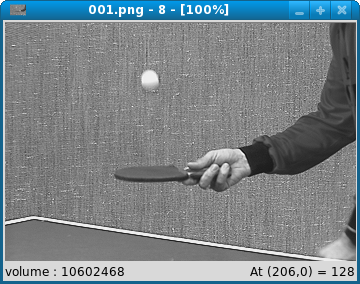
\includegraphics[scale=0.5]{images/dis2D.png}
\caption{2D display}
\label{fig:dis2D}
\end{figure}


\begin{figure}
\centering
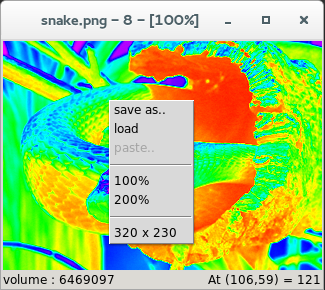
\includegraphics[scale=0.5]{images/dis2D_menu.png}
\caption{2D display: contextual menu}
\label{fig:dis2D_menu}
\end{figure}

A contextual menu is also available by right-clicking in the display. It offers
services like saving, opening, etc. Figure \ref{fig:dis2D_menu} shows an example of 
contextual menu. The first three choices are obvious. Then, you can choose a zoom
value between 100\% or 200\%. The last menu item indicates the size of
the image.

\subsubsection{3D display}

The 3D display is composed of three different approaches to display 3D images:
Volume rendering, projection and player. When you activate the 3D display,
you can dynamically switch between the three at your convenience.

\tipBox{
The foot data used for the display demo in this section can be found at
\url{http://tc18.liris.cnrs.fr/code_data_set/3D_images.html}
}

\paragraph{Projection display}

This display, see figure \ref{fig:dis3D_proj}, is basically an adaptation of
the 2D display. It is a basic plane projection along the three axis.
You can select this display by pressing key F1 on your keyboard.

\begin{figure}
\centering
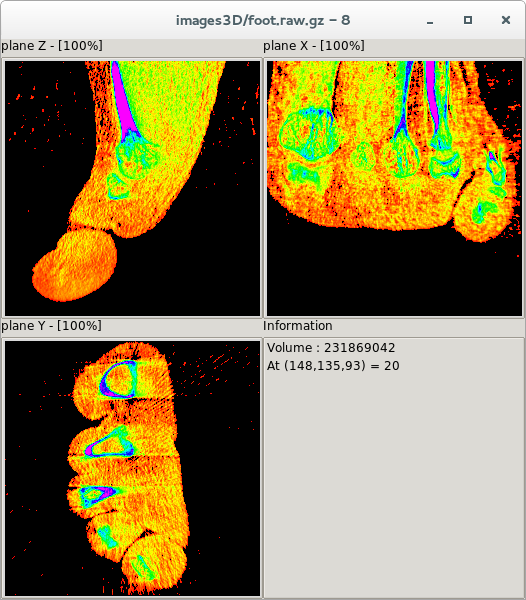
\includegraphics[scale=0.5]{images/dis3D_proj.png}
\caption{3D display: projection}
\label{fig:dis3D_proj}
\end{figure}

You can navigate through planes moving your mouse while holding <ctrl> down.
The mouse motion will allow you to change the plane following it (the displayer
shows a red cross to indicate where you are in the image data).

This is a more appropriate display if you need precision and careful
analysis of a result. However it only shows a limited amount of the
image at any given time.

\paragraph{Volume rendering display}

This display, see figure \ref{fig:dis3D_volren}, is ensured through the VTK
library and thus is only available if you have this library installed with
the Python bindings. Remind also that VTK is currently not available with Python 3. 
You can select this display by pressing key F2 on your keyboard.

\begin{figure}
\centering
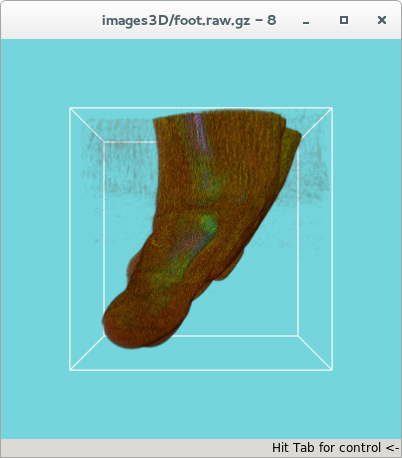
\includegraphics[scale=0.5]{images/dis3D_volren.png}
\caption{3D display: volume rendering}
\label{fig:dis3D_volren}
\end{figure}

The image is displayed inside its bounding cube and you can control its rotation
and zoom with your mouse.

This display comes with an integrated controller which allows you to change
the various options of display available. As shown in figure \ref{fig:dis3D_volren_ctrl},
you can change the opacity, the background color and the rendering methods.

The transparency/opacity of a pixel depends on its value. By clicking on the 
transparency bar, every pixel with value below will be transparent and above
pixels will be opaque.

To change the background, just click on the background bar. It will open a
color chooser dialog box in which you can pick up any background color you
might want.

\begin{figure}
\centering
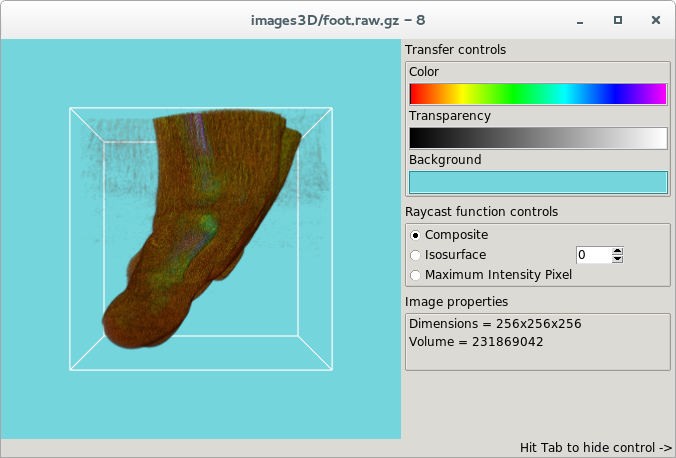
\includegraphics[scale=0.5]{images/dis3D_volren_ctrl.png}
\caption{3D display: volume rendering controls}
\label{fig:dis3D_volren_ctrl}
\end{figure}

Three distinctive methods to perform volume rendering can be selected:
\begin{itemize}
\item \textbf{Composite}: the result is a blend of all the pixels crossed by
the ray of light accordingly to their color and transparency.
\item \textbf{Isosurface}: the result shows only pixels with a given
value. It also uses shading to allow a better visualisation of the volume.
\item \textbf{Maximum Intensity Pixel (MIP)}: the result is the color and
transparency of the pixel with the highest value that the light ray hits.
\end{itemize}
You can see the results of the 3 different methods in figure 
\ref{fig:dis3D_volren_method}.

\begin{figure}
\centering
\begin{tabular}{ccc}
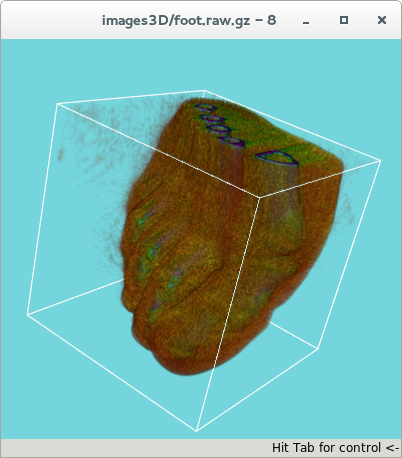
\includegraphics[width=0.25\textwidth]{images/dis3D_volren_compo.png} & 
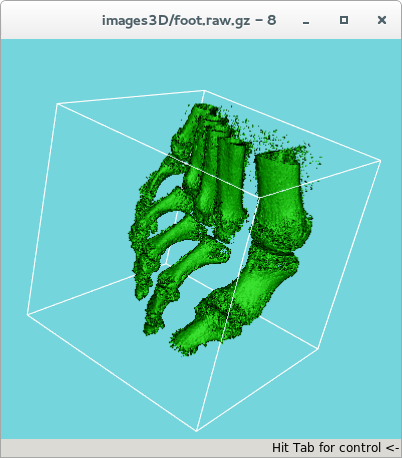
\includegraphics[width=0.25\textwidth]{images/dis3D_volren_iso.png} &
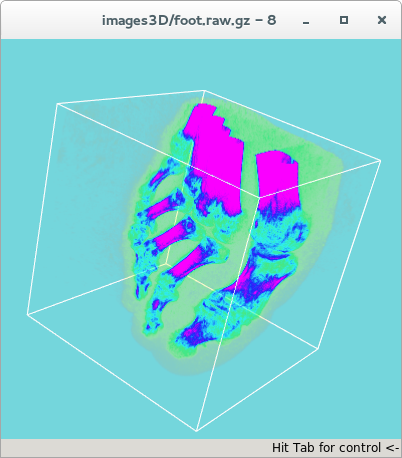
\includegraphics[width=0.25\textwidth]{images/dis3D_volren_mip.png} \\ 
Composite &
Isosurface &
MIP \\ 
\end{tabular}
\caption{3D display: volume rendering methods}
\label{fig:dis3D_volren_method}
\end{figure}

You can rotate (holding your mouse left button while moving it), zoom in and
out (same movement while holding the right button) and displace the image
(this time by holding both the left button and the shift key on your keyboard
while moving the mouse). This allows you to view more precisely any area of
your image. You can restore the initial settings by pressing r (Although this
does not seem to affect rotation).

We feel this display is appropriate to get an overall idea of your
result. However, it may lack precision and it could be troublesome to
understand what or where you are looking at. Use it cautiously.

\paragraph{Player display}

This display, see figure \ref{fig:dis3D_play}, will display the 3D image
as a sequence of 2D images that can be played as a movie.
You can select this display by pressing key F3 on your keyboard.

\begin{figure}
\centering
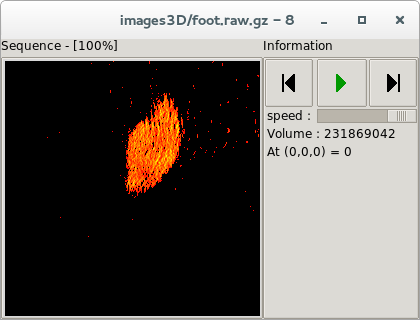
\includegraphics[scale=0.5]{images/dis3D_player.png}
\caption{3D display: player}
\label{fig:dis3D_play}
\end{figure}

The button allows you to play/stop or go to previous or next image in the
sequence. You can select the speed at which images are displayed.

\paragraph{3D displays particularities}
As you will see, unlike 2D images displays that are updated as the computations
progress, 3D images displays are not (for performance reasons). You will have
to update them manually by either hitting key F5 on your keyboard (with
the focus on the display you want to update) or call the update method.

We tried to provide Mamba3D with a coherent, useful and appropriate display.
However, contrary to 2D images, 3D images are difficult to represent on a 2D
display. Be sure to correctly configure the display before analysing results.

Lastly, as 3D images in Mamba3D are stacks of 2D images (imageMb objects), you 
always have the possibility to activate their own display at all time.

\lstset{language=Python}
\begin{lstlisting}
# Activates the display for slice number 128 of 3D image
im3D[128].show()
\end{lstlisting}

\subsubsection{Display control inside a script}
\label{cha:dis_arguments}

Image displays can be set and controlled inside a script (Mamba program) through the use
of some arguments inside the show() method.

The palette can be changed. For instance, changing the im palette to "rainbow"
can be performed by:

\lstset{language=Python}
\begin{lstlisting}
im.show(palette="rainbow")
\end{lstlisting}

Returning back to the default palette (grey) can be achieved by:

\lstset{language=Python}
\begin{lstlisting}
im.show(palette=None)
# This also works...
im.show(palette="")
\end{lstlisting}

The zoom value can be set with the zoom argument. For instance:

\lstset{language=Python}
\begin{lstlisting}
im.show(zoom=1.5)
\end{lstlisting}

It is also possible to move the zoomed image with the argument at=(x,y), (x,y) being
a tuple defining the origin of the zoomed part (it is similar to a displacement of the
scroll bars of the display window). Both arguments can be used simultaneously:

\lstset{language=Python}
\begin{lstlisting}
im.show(zoom=2, at=(50,60))
\end{lstlisting}

When displaying 32-bit images, the plane argument allows to select the byte plane (from 0 to 3) among the
four ones which will be displayed:

\lstset{language=Python}
\begin{lstlisting}
im32.show(plane=2)
\end{lstlisting}

To come back to the whole display, enter:

\lstset{language=Python} 
\begin{lstlisting}
im32.show(plane=4)
\end{lstlisting}

Regarding 3D images, there exists three different display modes in Mamba: VOLUME, PROJECTION
and PLAYER (for image sequences which are considered in Mamba 2 as 3D images). Each mode can be set up
by using the mode argument:

\lstset{language=Python}
\begin{lstlisting}
# This mode enables the 3D rendering display (provided that VTK is properly installed)
im32.show(mode="VOLUME")
\end{lstlisting}

Any string other than the three mentioned above enables the default display (PROJECTION).

\subsubsection{Display shortcuts}
\label{cha:dis_shortcuts}

There are numerous possibilities to interactively control displays. Here is a list of
keyboard shortcuts available in the various displays:

\begin{itemize}
\item \textbf{P}: will circle through all the available palettes.
\item \textbf{Z} and \textbf{A}: will zoom in/out in 2D displays (basic, 
projection, player ...)
\item \textbf{B} and \textbf{N}: With 32-bit images, these keys will allow you
to move through byte planes or to show the complete image downscaled.
\item \textbf{Control-F}: will freeze/unfreeze the display. See the freeze() 
method.
\item \textbf{Control-R}: will reset the display to its original size and
zoom value.
\item \textbf{Control-V}: will copy any image stored inside the clipboard 
in your image (only works on 2D images on Windows platforms).
\item \textbf{F1}: on a 3D image display, will switch to PROJECTION mode.
\item \textbf{F2}: on a 3D image display, will switch to VOLUME mode
if you have VTK Python bindings available on your computer.
\item \textbf{F3}: on a 3D image display, will switch to PLAYER mode.
\item \textbf{F5}: on a 3D image display, will update the display with
the image content. Similar to the method update.
\item \textbf{Space} : will start/stop the player in the 3D image display
PLAYER mode.
\item \textbf{Page-Up} : will display the next image in the sequence in the
3D image display PLAYER mode.
\item \textbf{Page-Down} : will display the previous image in the sequence
in the 3D image display PLAYER mode.
\end{itemize}

You can also use your mouse:

\begin{itemize}
\item \textbf{scrolling} : will zoom in/out in 2D displays (basic, 
projection, player ...)
\item \textbf{motion+Control} : will allow to move through the image
in the 3D image display PROJECTION mode.
\end{itemize}

\subsubsection{Palettes and other display functions}
\label{cha:pal}

As you have seen above, you can activate palette through shortcut P when displaying
images. Mamba comes with four preintegrated palettes : "rainbow", "inverted rainbow",
"patchwork" and "heat view".

You can create your own palette using the functions offered in package
mambaDisplay.

\lstset{language=Python}
\begin{lstlisting}
import mambaDisplay

# Creates a palette to emphase one specific pixel value
# Here the 255 valued pixels will be seen in red.
mambaDisplay.tagOneColorPalette(255, (255,0,0))
# Once created the palette is available through the P shortcut
# under the name 'tag 255 (255,0,0)'

# You can also add your own palette
mambaDisplay.addPalette("my own palette", my_own_palette)
# where my_own_palette is a tuple containing 256*3 values (r0,g0,b0,r1,g1,b1 ...)
\end{lstlisting}

Palette can also be used with the save method to colorize the saved image.

Sometimes, you will have lots of images opened and displayed making it quite
messy on your desktop and thus very difficult to read and analyze. There are a
bunch of methods and functions to help you organise your displays.

Firstly, you can give a name to your image that will be displayed in the window
title making it easier to know what is represented by the display:

\lstset{language=Python}
\begin{lstlisting}
# Setting im name to 'result'
im.setName('result')
\end{lstlisting}

When the screen gets filled with lots of displays, it can be excruciatingly
boring and slow to order all of them so that they don't overlap. To make sure 
displays are properly and automatically organised, you can call the following 
function in the mambaDisplay package:

\lstset{language=Python}
\begin{lstlisting}
mambaDisplay.tidyDisplays()
\end{lstlisting}

The function does not do miracles (like increasing your screen resolution) so
don't have too much expectations.

Large and small images are not displayed at their original size but they are
zoomed in (if they are too small) or zoomed out (if they are too large). By
default, images larger than 512 in width or height are zoomed out by a factor 2
until the size of the zoomed out displayed image is below this maximum value.
In the same way, an image smaller than 256 will be zoomed in (x2) until
the displayed image is larger than this minimum. For instance, a 1024x1024 image
will be displayed after a zoom-out equal to 25\% whereas a 200\% zoom-in will be
applied on a 128x128 image.

The default values of the display sizes can be changed by means of the following
functions:

\lstset{language=Python}
\begin{lstlisting}
mambaDisplay.setMaxDisplay(size)
mambaDisplay.setMinDisplay(size)
\end{lstlisting}

where size is a tuple containing the upper (in setMaxDisplay) or lower (in
setMinDisplay) limits of the width and height of the display.
These functions belong to the mambaDisplay package. It is wise to use them at
start before displaying any image. Under Windows, these functions could be put
in the \_init\_.py file of the Mamba shell (see section \ref{cha:mamba_shell}).

\lstset{language=Python}
\begin{lstlisting}
# Setting display max size to (800,800)
import mambaDisplay
mambaDisplay.setMaxDisplay((800,800))
\end{lstlisting}

\subsubsection{Extra displays}

A specific module has been created to offer some extra display methods.

The module mambaDisplay.extra offers functions to display, interact and generally 
perform operations that need the constant intervention of the programmer. For
example, this module provides an interface to allow dynamic threshold of a given
image (threshold value can then be modified on the fly by the user).

This module is not automatically imported and needed to be imported manually if
you want to use it.

\lstset{language=Python}
\begin{lstlisting}
# Importing the mambaDisplay.extra module
from mambaDisplay.extra import *
\end{lstlisting}

A greyscale or 32-bit image can be thresholded interactively with the
\textbf{dynamicThreshold} operator. This operator opens a window (figure \ref{fig:inter_thresh})
displaying the binary thresholded image. The threshold values can be modified by hitting
Q, W, S and X on the keyboard. See the documentation for further details.

\begin{figure}
\centering
\begin{tabular}{cc}
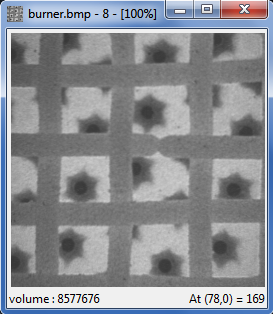
\includegraphics[width=0.4\textwidth]{images/burner.png} & 
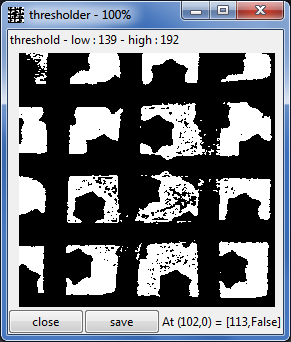
\includegraphics[width=0.4\textwidth]{images/thresholder.png} \\ 
Original &
Threshold \\ 
\end{tabular}
\caption{Interactive thresholding of the left Burner image}
\label{fig:inter_thresh}
\end{figure}

On exit (when hitting the close button), the operator returns a list containing the
threshold values.

\lstset{language=Python}
\begin{lstlisting}
# Interactive thresholding
from mambaDisplay.extra import *
im.loadimage("Burner.png")
dynamicThreshold(im)
# When exiting, we get:
[139, 192]
\end{lstlisting}

The \textbf{superpose} operator, when launched, displays, superposed in the same window, either
a greyscale or 32-bit image and a binary one, or two binary images. The color of the
binary displays can be modified by clicking the color buttons (figure \ref{fig:superpose}). 

\begin{figure}
\centering
\begin{tabular}{cc}
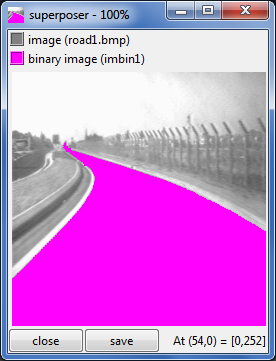
\includegraphics[width=0.4\textwidth]{images/superposer.png} & 
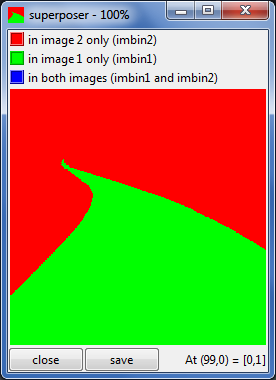
\includegraphics[width=0.4\textwidth]{images/binsuperposer.png} \\ 
Greyscale and binary image &
Two binary images \\ 
\end{tabular}
\caption{Superposing a greyscale and a binary image (left) or two binary images (right)}
\label{fig:superpose}
\end{figure}

The \textbf{interactiveSegment} operator allows to interactively segment a 8-bit or 32-bit
image with the watershed transform by injecting manually markers on it. Each new marker modifies
the segmentation (figure \ref{fig:inter_segment}). On exit, this operator returns a list of markers
coordinates.

\lstset{language=Python}
\begin{lstlisting}
# Launching interactive segmentation
from mambaDisplay.extra import *
interactiveSegment(im, im32)
\end{lstlisting}

The 32-bit im32 image contains the watershed segmentation.

\begin{figure}
\centering
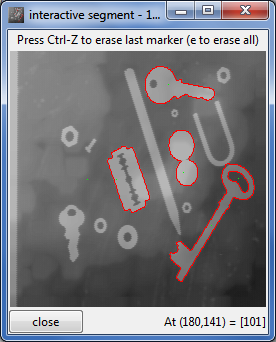
\includegraphics[scale=1.0]{images/interactiveSegment.png}
\caption{Interactive segmentation}
\label{fig:inter_segment}
\end{figure}

\subsection{Structuring elements}

 \subsubsection{Defining structuring elements}
 
Two of the most important operations of mathematical morphology: erosion and
dilation (functions erode and dilate and their 3D counterpart respectively)
are based on a structuring element which controls the behavior of the operator.

\label{cha:structelem}
2D structuring elements are instances of the \textbf{structuringElement} class,
while 3D ones are instances of the \textbf{structuringElement3D}
class. Remember also that a \textbf{doubleStructuringElement} and a
\textbf{doubleStructuringElement3D} classes exist. They are used with
the thinning and thickening operators.

Each structuring element is associated to a grid. It is defined by the neighbors
of the central point it contains. Its origin is always
the central point, even when this point does not belong to the structuring element.

The class structuringElement allows you to describe a structuring element to
be used with the erode and dilate functions. This class can only describe
structuring elements that are included in the local 
neighbors of the central point (adjacent points).

\begin{figure}
\centering
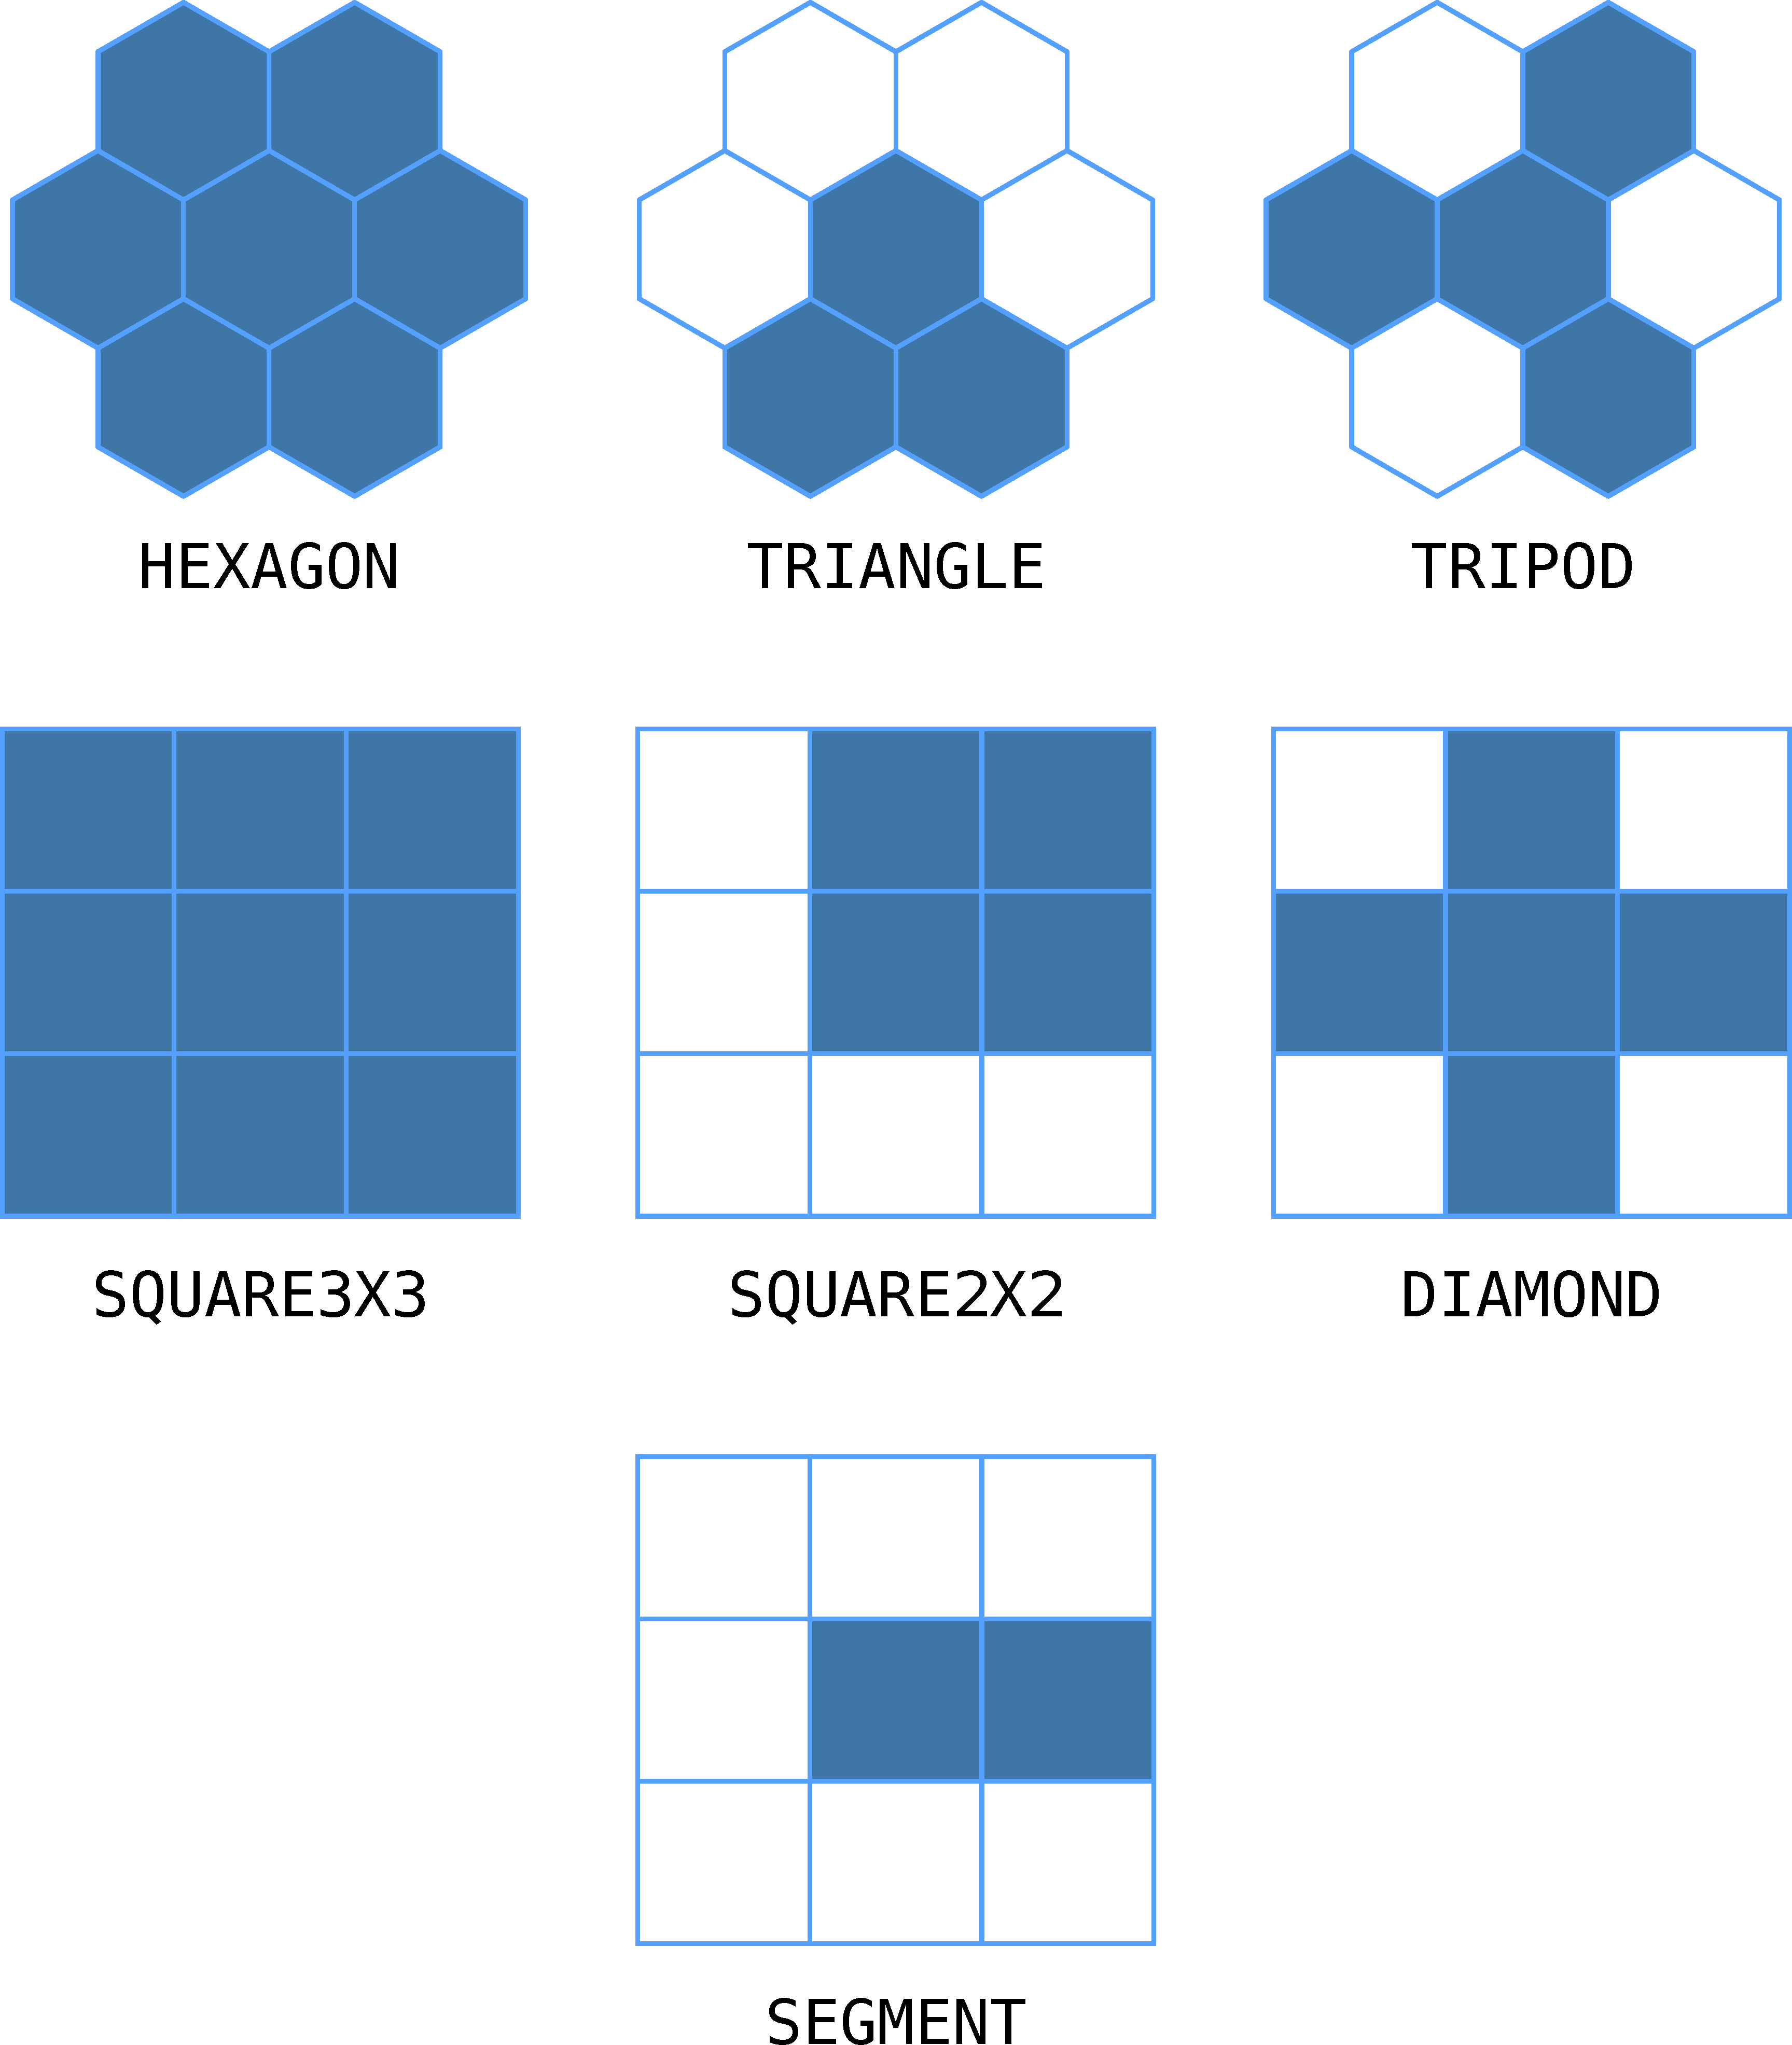
\includegraphics[width=0.4\textwidth]{figures/se.pdf}
\caption{Structuring elements defined in Mamba}
\label{fig:se}
\end{figure}

Mamba includes some of the most usual structuring elements. Figure
\ref{fig:se} gives their list and representation.

You can define your own structuring element easily. To do so you will need to
identify the grid it is based on and the points that you want to include 
inside your structuring element. Refer to figures \ref{fig:hxgriddir} and 
\ref{fig:sqgriddir} for neighbors coding values. Here is an example:

\lstset{language=Python}
\begin{lstlisting}
# Creating a reverse triangle
reverse_triangle = structuringElement([0,1,6], HEXAGONAL)

# performing an erosion with the created structuring element
erode(imIn, imOut, 1, se=reverse_triangle)
\end{lstlisting}

\warnBox{
Some erosion and dilation functions implemented in Mamba do not use this
structuring element class for performance or feasability reasons.
}

\warnBox{
Be also aware that, when you are combining operations using a structuring element
and operations using a grid, you may have discrepancies between the internal grid used
in the structuring element and the grid you used as an argument (or the default). To
prevent this, use the getGrid() method of the structuring element class. See also section \ref{cha:rules}.
}

Mamba3D predefined five structuring elements to be used with the appropriate
3D operators:

\begin{itemize}
\item \textbf{CUBIC3X3X3} : A three pixels large cube. Based on the CUBIC grid.
\item \textbf{CUBIC2X2X2} : A two pixels large cube. Based on the CUBIC grid.
\item \textbf{CUBOCTAHEDRON1} : A first cuboctahedron. Based on the
FACE\_CENTER\_CUBIC grid (see figure \ref{fig:cuboc_fcc}).
\item \textbf{CUBOCTAHEDRON2} : A second cuboctahedron. Based on the
CUBIC grid (see figure \ref{fig:cuboc_c}).
\item \textbf{CUBOCTAHEDRON3} : A third cuboctahedron. Based on the
CENTER\_CUBIC grid (see figure \ref{fig:cuboc_cc}).
\end{itemize}

\begin{figure}
\centering
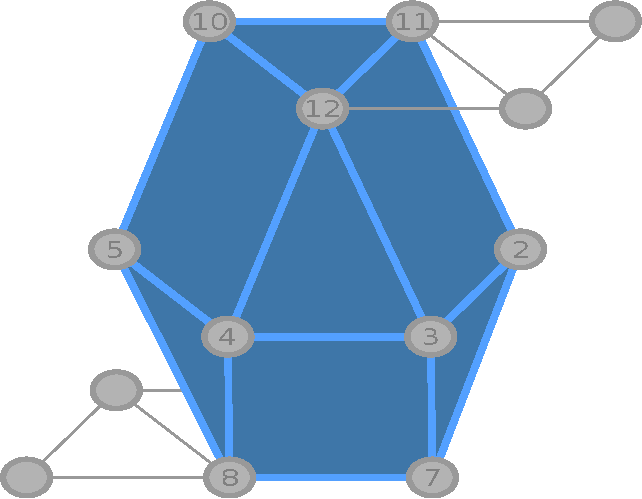
\includegraphics[width=0.4\textwidth]{figures/Cuboc_on_fccubic.pdf}
\caption{Cuboctahedron defined on the face centered cubic grid}
\label{fig:cuboc_fcc}
\end{figure}

\begin{figure}
\centering
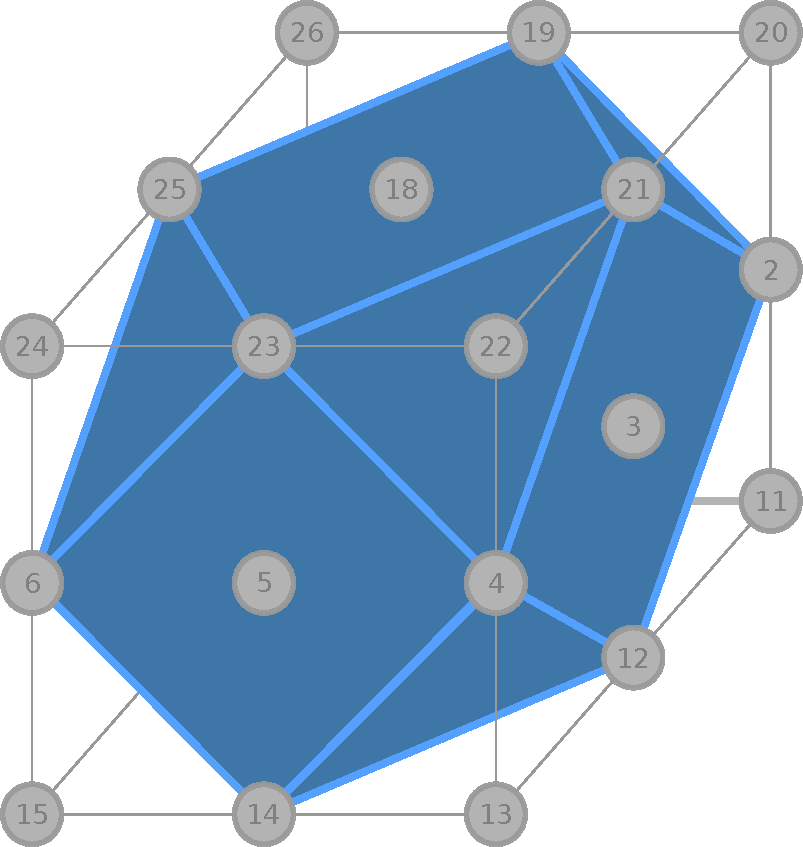
\includegraphics[width=0.4\textwidth]{figures/Cuboc_on_cubic.pdf}
\caption{Cuboctahedron defined on the cubic grid}
\label{fig:cuboc_c}
\end{figure}

\begin{figure}
\centering
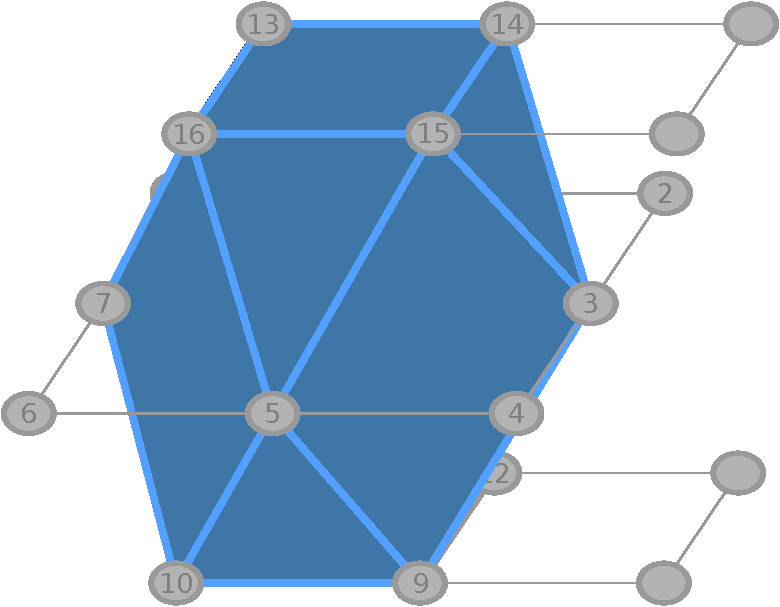
\includegraphics[width=0.4\textwidth]{figures/Cuboc_on_ccubic.pdf}
\caption{Cuboctahedron defined on the centered cubic grid}
\label{fig:cuboc_cc}
\end{figure}

Note that the orientation and size of the different cuboctahedrons are different
in the three grids.

You can also, of course, create your own structuring elements:

\lstset{language=Python}
\begin{lstlisting}
# Creating a small pyramid
pyramid = structuringElement3D([0,1,2,3,14], CENTER_CUBIC)

# Why not a tetrahedron
tetrahedron = structuringElement3D([0,1,2,11], FACE_CENTER_CUBIC)

# You can of course build pyramids and tetrahedrons with
# different directions. The next two are a bit better because they
# are centered
pyramid2 = structuringElement3D([0,9,10,11,12], CENTER_CUBIC)
tetrahedron2 = structuringElement3D([0,7,8,9], FACE_CENTER_CUBIC)
\end{lstlisting}

\subsubsection{Structuring element methods}

 Different methods exist to deal with these 2D and
3D structuring elements: \textbf{getGrid} returns the grid associated with the structuring element, \textbf{getDirections} returns the
directions used by the structuring element (with or without direction 0), \textbf{hasZero} indicates if the structuring element contains
or not the central point, etc.
In 2D, a major difference between Mamba 1.x and Mamba 2.x lies in the way directions are defined and used in the \textbf{infNeighbor}, \textbf{supNeighbor}
and \textbf{diffNeighbor} operators. It is now possible to use several directions at the same time. These directions, however, must be coded.
This coding is performed by the \textbf{getEncodedDirections} method. All the directions \emph{i} of the structuring element \emph{se} are used to define a
number \emph{nb} equal to:

\begin{displaymath}
nb = \sum_{i \in se} 2^i
\end{displaymath}

which is actually used by the operators. The main advantage of this approach is a dramatic increase of the computation speed of the basic
morphological transforms (erosion, dilation). Here are examples of direction encoding for some common structuring elements:

\lstset{language=Python}
\begin{lstlisting}
>>> HEXAGON.getEncodedDirections()
127
>>> HEXAGON.getEncodedDirections(withoutZero=True)
126
>>> TRIANGLE.getEncodedDirections()
25
\end{lstlisting}

In 3D, the same encoding is needed. But, as the structuring elements can be defined on three 2D layers, this encoding is performed on each
one so that the basic 3D erosions and dilations can be obtained rapidly by performing partial operations on each plane of the 3D image and by
combining these partial results. This encoding is performed by the \textbf{getEncodedDirs} method which returns a dictionnary containing the 2D
structuring elements encodings for the three sections of a given 3D structuring element. The result obviously depends of the \emph{z} position of the
structuring element:

\lstset{language=Python}
\begin{lstlisting}
>>> dirs = CUBOCTAHEDRON1.getDirections()
>>> CUBOCTAHEDRON1.grid.getEncodedDirs(dirs, 0)
{0: 127, 1: 67, -1: 97}
>>> CUBOCTAHEDRON1.grid.getEncodedDirs(dirs, 1)
{0: 127, 1: 49, -1: 25}
>>> CUBOCTAHEDRON1.grid.getEncodedDirs(dirs, 2)
{0: 127, 1: 13, -1: 7}
\end{lstlisting}

\subsection{Mamba Shell}
\label{cha:mamba_shell}

\textbf{Only on Windows}

The Mamba Shell is in fact a simple shortcut to IDLE, the standard Python shell
integrated into a Tkinter GUI. This shortcut serves three purposes:

\begin{itemize}
\item Make sure IDLE is started with the correct options to run properly Mamba
(see section \ref{cha:lim_restrict}).
\item Make it easy for beginners to start Mamba by providing them a shortcut
to a fully working environment with preloaded modules and packages.
\item Make it easy for advanced users to customize their default environment
(number of loaded images, size, particular imports ...) by editing an appropriate
file.
\end{itemize}

\tipBox{
If you are not using IDLE as your Python environment, you can still benefit
from the mambaShell by simply importing it inside your own Python shell.
The syntax "from mambaShell import *" is strongly advised for easier use.
}

\subsection{Regarding optimizations}

\tipBox{
If you are trying to optimize your algorithm, the Python reference documents
will be useful to obtain information on how functions operate and what
sort of performance is to be expected. See section \ref{cha:other_docs}.
}

Mamba is a very large library implementing a lot of functions. Consequently, it
is likely there is more than one way to create your algorithm using the functions
provided by the library. However, among all these possibilities, one is surely more
fitted to your purpose (as regards code clarity and comprehension, speed, size ...).

Regarding speed, you will likely have to study extensively the various
available functions. Mamba always tries to implement the fastest function to 
perform any task. However, sometimes other constraints (like readability and
simplicity) gets in the way of the fastest implementation.

For example, consider the opening by build of an image. The openByBuild function
found in the mamba package is appropriate to perform this operation and
is as fast as possible if it has to work with all image depths indiscriminately.
This operator uses the build function which works with any image
depth. However, there exists a faster reconstruction operator,
hierarBuild, which works with non binary images (8-bit or 32-bit). Therefore, if you
know that you are only using greyscale or 32-bit images, it might be a good idea to create
your own openByBuild function like this:

\lstset{language=Python}
\begin{lstlisting}
import mamba

def openByBuild_greyscale(imIn, imOut, n=1, se=mamba.DEFAULT_SE):
    """
    Performs an opening by reconstruction operation on image 'imIn' and puts the
    result in 'imOut'. 'n' controls the size of the opening.
    
    This function only works for greyscale or 32-bit images and is an optimization of
    openByBuild.
    """
    
    imWrk = mamba.imageMb(imIn)
    mamba.copy(imIn, imWrk)
    mamba.erode(imIn, imOut, n, se=se)
    mamba.hierarBuild(imWrk, imOut, grid=se.getGrid())
\end{lstlisting}

In other cases, Mamba will offer two functions performing the exact same 
operation with identical results but doing it with two algorithms presenting
different performance characteristics.

Consider the case of erosion using an hexagon. Two functions exist in Mamba to
perform this operation: erode and largeHexagonalErode.

\lstset{language=Python}
\begin{lstlisting}
# Erosion of imIn by an hexagon of size 1 put into imOut
erode(imIn, imOut, 1, se=HEXAGON)
largeHexagonalErode(imIn, imOut, 1)
\end{lstlisting}

In the example above, the result is the same for both functions. However, erode is
more than two times faster than largeHexagonalErode. But in this case:

\lstset{language=Python}
\begin{lstlisting}
# Erosion of imIn by an hexagon of size 20 put into imOut
erode(imIn, imOut, 20, se=HEXAGON)
largeHexagonalErode(imIn, imOut, 20)
\end{lstlisting}

largeHexagonalErode is this time more than two times faster than erode. You will
have to take into account this particularities when implementing your algorithm
if you want to speed it up. Regarding largeHexagonalErode, refer to section 
\ref{cha:opt_ero_dil} for more information.

\pagebreak

\subsection{Further information regarding Mamba3D}

\subsubsection{Computations/Functions}

Performing computations with Mamba3D was meant to be as close as possible
as the way they are done in Mamba. Thus function names are identical except
for a postfix "3D" indicator.

\lstset{language=Python}
\begin{lstlisting}
# For example the erode function in Mamba
erode(imIn, imOut, n=1, se=DEFAULT_SE, edge=FILLED)
# will become in Mamba3D (beware of the mamba.FILLED needed if you did 
# not import mamba)
erode3D(imIn, imOut, n=1, se=CUBOCTAHEDRON1, edge=mamba.FILLED)
\end{lstlisting}

Although it might seem bothersome to add the "3D" postfix to every
function you are using when computing in 3D, it is also needed to be able to
use both the 2D functions and their 3D counterpart in the same script.

This naming convention was also adopted, for the most part, by module
names in the Mamba3D package.

As simple as it is, you will still face difficulties if you try to translate
your 2D algorithm into 3D. First, computations take more time (see section
\ref{cha:perfo3D}) but Mamba3D does not offer all the functions found in
the Mamba API. The section \ref{cha:missing3D} describes some of the 
main differences between the two.

\subsubsection{Performance discussion}
\label{cha:perfo3D}

Performing computation on 3D data is performance consuming. For example, if
you compare a 2D erosion with a hexagonal structuring element versus a 3D
erosion using a cuboctahedron structuring element, you will have to perform
twice more operations per pixel in the later. If you take into account that
the number of pixels is also greater in 3D (and not by a small amount), you end
up with a very large difference of speed between the two operations.

Thus, if you need to process 3D images, you get only three choices, get patient, 
get a faster computer or code a library fully optimized for 3D operations 
(which Mamba3D isn't).

Another performance problem arises with the display. VTK is a very powerful
library offering state of the art methods and algorithms to display 
data of all kinds. Mamba3D uses the volume rendering techniques based on 
\textbf{CPU computation and not GPU} implemented into VTK. Of course, they
are slower than the ones using the GPU but they do not require a modern
graphic card. Feel free to modify the source code of Mamba3D to use the
GPU volume rendering methods. Other displays are less greedy but they
are still more CPU consuming than a simple 2D display.

Last but not least, memory consumption will also be dramatically more important
in Mamba3D but that goes without saying.

\subsubsection{Missing or reduced operators}
\label{cha:missing3D}

As you will see, Mamba3D does not completely translate the Mamba API into
a 3D version of it. There are still some missing operators. Here is a non
exhaustive list of 2D operators that have not been transposed in Mamba 3D yet.
Some of them could be added in the future. For some others (rotating thinnings
and thickenings in particular), it is unlikely that they will be translated, as
this would be a really difficult challenge.

\begin{itemize}
\item Most of the operators in mamba module thinthick (except the basic ones).
\item Some operators in mamba module largeErodil, especially those using 3D Steiner polyhedra (except
for the cube).
\item All the operators in mamba module residues.
\item All the operators in mamba module hierarchies.
\item Some of the operators in mamba module measure.
\end{itemize}

Some operators do not work in Mamba3D exactly as in Mamba.

\begin{itemize}
\item structuringElement3D offers no method to rotate them.
\end{itemize}

This is not the complete list and if you have any doubt about the behavior
of a function, we advise you to go and look at its documentation.

\pagebreak

\section{Add-ons and extensions}
\subsection{mambaRealtime}

The Mamba Realtime module is an extension to the Mamba library for Python that 
allows you to test your algorithms on realtime acquired images.

The Mamba library allows you to develop easily and rapidly applications based on 
mathematical morphology algorithms. 

Most of the time, you will test and try your ideas on static images to make sure 
that your algorithm is working correctly and efficiently. However, as good as 
this approach might be, it still lacks something when you want to confront your 
algorithm to "dynamic real life situation", meaning noise, unpredictable 
movement, fast input, etc ... that your algorithm will have to handle to 
efficiently work in a realtime situation.

The Mamba Realtime was built to help you test these situations easily without 
having to recode your algorithm in another language.

Currently two versions of this module exist, one for Windows platforms and 
another for Linux platforms. It offers the following services :

\begin{itemize}
\item Acquire images from supported image acquisition device (Video 4 Linux 2
devices on Linux or DirectShow devices on Windows). Currently, this means that
most of the webcams are 
supported.
\item Retrieve images from video sources using the FFmpeg library (lots of video
codecs are supported).
\item Display the result of your algorithm in realtime.
\item Record the result using the FFmpeg library.
\end{itemize}

\warnBox{
Please note that the Mamba Realtime module is \textbf{NOT} released under 
the same license. Currently this module is under GPL. Consult the appropriate
documentation for more information.
}

\warnBox{
Note also that the Mamba Realtime module is \textbf{NOT} does not work properly on 
any 64-bit Windows environment. Therefore, we advise you to use Linux if you
intend to use this add-on.
}

For more information regarding this add-on, refer to the appropriate document.

\pagebreak

\section{Limitations and restrictions}
\label{cha:lim_restrict}

Unfortunately, Mamba has some built-in limitations that may be corrected later
but that you will have to deal with in the meantime.

Whatever image you load, it will always be assumed that it is a greyscale image.
By default, Mamba uses the ITU-R 601-2 luma transform to convert color images 
into greyscale images. You can of course specify your own transformation matrix 
(refer to the Python and Pillow reference documentations).

Mamba is known to have some troubles with IDLE. Mamba uses
Tkinter for image display and this may produce interferences with IDLE. The
problem is known to occur when IDLE is run with subprocess enabled which is the
default mode when IDLE is invoked through the Windows main menu. However, there 
is no problem when IDLE is started with no subprocess (option -n) as, for 
example, when right-clicking on a Python file and selecting "Edit with IDLE" from
the contextual menu. IDLE will display a short sentence if subprocesses are
deactivated before the first shell prompt. So if you want to use IDLE, you have
three options:

\begin{itemize}
\item Start IDLE with subprocess disabled (option -n). This will allow you to 
use Mamba display but unfortunately will prevent you using the integrated
debugger. The Mamba Shell on Windows is in fact a shortcut to do this.
\item Start IDLE with subprocess enabled (default mode on Windows) but do not
use Mamba standard display. This way you have access to the integrated debugger.
\item Install Mamba with the IDLE shell and launch MambaShell at startup (see
section \ref{cha:mamba_shell}).
\end{itemize}

In any case, Mamba should work perfectly with the standard Python shell 
(command line).

Along those problems with IDLE, you can also face difficulties when using
Mamba with other GUI libraries. Indeed, when using the embedded display,
Mamba relies on the PyOS\_InputHook trick. It allows the Python shell (where 
you type all your commands) to still be operational while at the same time
processing GUI events (such as mouse clicks keyboard inputs ...). When you
start any Mamba display, Tkinter grabs the hook thus making it unavailable
for other libraries which might need it. Similarly if Mamba is started
after a library that has grabbed the hook, the embedded display will not
work (display will be frozen). In particular, if you are a user of pylab,
make sure to import it \textit{after} Mamba because it is likely
this library will grab the hook (you must do this only if your intention is to
display Mamba images). It is not sure we will be able to fix this in a near
future. However, as long as you don't need to use the display, Mamba should 
work fine with any other library.

\pagebreak

\section{Other documents and references}
\label{cha:other_docs}

Mamba documentation is pretty large and covers C API, Python API, user manual 
and add-ons documentation. Here is a list of these documents and what 
information you can find in them:

\begin{itemize}
\item \textbf{\textsc{mamba C API Reference Manual}}: This document refers to the
low-level C API. It is generated using sources code and Doxygen. If you intend 
to modify the C functions, this document may be useful to you. It gives some
explanations regarding the image data structure used inside Mamba. Have also
a look at section \ref{cha:lib_arch} for general information regarding Mamba
architecture.
\item \textbf{\textsc{Mamba Image Library Python Reference}}: As soon as you
start using Mamba, you will need to keep this document close to you. All the
Python functions present in Mamba are explained in this document. It gives
information on how to use them, what sort of result to expect and so on... 
\item \textbf{\textsc{Mamba API quick reference}}: This document is the very
compacted version of the previous one. All the functions listed on the shortest
possible number of pages plus some of the more useful pieces of information you
might need. This quick reference is meant to help you quickly remember function
name and arguments but it can also be useful to get to know all the functions
implemented in Mamba.
\item \textbf{\textsc{Mamba Image Examples}}: This document describes various
examples regarding how to use Mamba and the kind of results you can expect.
\end{itemize}

\pagebreak

\section{Algorithmic approaches in Mamba}

Some of the operators included in Mamba are based on specific algorithms.
In this section, we list some of them and give references to the articles or 
courses that describe them. You can also take a glimpse inside the sources to
see how they were implemented.

\subsection{Hierarchical lists : Watershed and Build}

Mamba is using hierarchical lists to perform watershed computations and some
particular build operators.

The use of hierarchical lists for watershed was first described in a patent 
document. This article described mainly an algorithm to extract basins.

\begin{enumerate}
\setcounter{enumi}{0}
\item \label{art:meyer} Fernand Meyer,
\emph{Image processing method by hierarchical queues},
Available at \url{http://www.freepatentsonline.com/EP0576584.html}, 1992
\end{enumerate}

More details for a similar algorithm allowing to extract an idempotent 
watershed line can be found in the following article.

\begin{enumerate}
\setcounter{enumi}{1}
\item \label{art:beucher2} Serge Beucher, Nicolas Beucher,
\emph{Hierarchical queues implementation: general description and enhancements
in Mamba software library},
Available at \url{http://cmm.ensmp.fr/\~beucher/Mamba\_documentation.html},
(to be published)
\end{enumerate}

Mamba implements these algorithms in the C core library for performance sake.
If you are interested, you can find them in the sources in files:

\begin{itemize}
\item \textbf{mambaApi\_loc.h}: The data structures used to represent the 
hierarchical lists in Mamba are described in this file.
\item \textbf{MB\_Basins.c}: A simple implementation of the hierarchical queues
to extract basins using a marker image for flooding wells. This is the simplest
use of hierarchical lists that is done in Mamba.
\item \textbf{MB\_Watershed.c}: An implementation of the hierarchical queues to
extract basins and watershed lines using a marker image for flooding wells.
\end{itemize}

Build (and its dual) operation can be performed using hierarchical queues in
Mamba by calling the appropriate functions. The implementation refers to
\ref{art:beucher2}.

Here is the list of source files implementing these operators. They are based on
the same data structures for the hierarchical lists as watershed operators:

\begin{itemize}
\item \textbf{MB\_HierarBld.c}: Implementation of the build operator for
greyscale images using the hierarchical lists.
\item \textbf{MB\_HierarDualBld.c}: Implementation of the dual build operator
for greyscale images using the hierarchical lists.
\end{itemize}

\subsection{Labelings}

The labeling algorithm implemented in Mamba employs a version of the union-find 
algorithm.

\begin{enumerate}
\setcounter{enumi}{2}
\item \label{art:wikipedia} Wikipedia Free Encyclopedia, 
\emph{Connected component labeling},
Available at \url{http://en.wikipedia.org/wiki/Connected\_Component\_Labeling}, 2007
\end{enumerate}

The code source implementing this algorithm can be found in the C core library
in file \textbf{MB\_Label.c}.

Other labeling operators can be found in the labelling.py module. They are described in \ref{art:beucher4}.

\begin{enumerate}
\setcounter{enumi}{3}
\item \label{art:beucher4} Serge Beucher,
\emph{Labelling Operators},
Available at \url{http://cmm.ensmp.fr/\~beucher/Mamba\_documentation.html}, 2014
\end{enumerate}

\subsection{Large erosions and dilations}
\label{cha:opt_ero_dil}

Erosion and dilation are quite common in mathematical morphology and thus Mamba
implements many variations of them to give you access to the most powerful ones.

\begin{enumerate}
\setcounter{enumi}{4}
\item \label{art:beucher1} Serge Beucher,
\emph{Fast implementation of large erosions and dilations in Mamba},
Available at \url{http://cmm.ensmp.fr/\~beucher/Mamba\_documentation.html}, 2010
\end{enumerate}

\ref{art:beucher1} describes an algorithm to perform large erosions and
dilations faster than with the standard method by repeating over a simple
operator. These algorithms are implemented in the large erosion and dilation
functions in Mamba. You can found them in module \textbf{erodilLarge.py} of
the mamba package and a reduced set of them adapted to 3D images in the
\textbf{erodilLarge3D.py} module.

\subsection{Hierarchical segmentations}
\label{cha:hierar_seg}

Mamba implements multiple algorithms performing segmentations based on
a hierarchization of an initial watershed.

\begin{enumerate}
\setcounter{enumi}{5}
\item \label{art:marcotegui_beucher} Serge Beucher, Beatriz Marcotegui
\emph{P algorithm, a dramatic enhancement of the waterfall transformation},
Available at \url{http://cmm.ensmp.fr/~beucher/publi.html}, 2009

\item \label{art:beucher3} Serge Beucher
\emph{Towards a unification of waterfalls, standard and P algorithms},
Available at \url{http://cmm.ensmp.fr/~beucher/publi.html}, 2012
\end{enumerate}

\ref{art:marcotegui_beucher} and \ref{art:beucher3} describe algorithms
implemented in module \textbf{hierarchies.py} of the mamba package.

\subsection{Working with partitions}
\label{cha:partitions}

A module, named \textbf{partitions.py}, provides basic and less basic
morphological transforms applied on partitions which can be considered as a dual representation
of a graph: each cell of the partition corresponds to a node of the graph and acts as a whole
(it is sometimes called a super-pixel).

\begin{enumerate}
\setcounter{enumi}{7}
\item \label{art:beucher4} Serge Beucher
\emph{Basic Morphological Operators Applied On Partitions},
Available at \url{http://cmm.ensmp.fr/~beucher/publi.html}, 2013
\end{enumerate}

\ref{art:beucher4} describes the various operators implemented in
module \textbf{partitions.py} of the mambaComposed package.

\pagebreak

\section{Extending and customizing Mamba}

Mamba is open-source so, if you want to modify/extend it, you are welcome. The
following section will present some aspects you might find useful in this
prospect. This section intended audience is advanced users who want to go 
further with Mamba. If you want to share your extensions of Mamba with other users,
have a look to the coding rules and standards in appendix \ref{cha:rules}. 

\subsection{Library architecture and design}
\label{cha:lib_arch}

Mamba is based on a very simple architecture. If you are going to modify it or
if you want to know more about it, reading this section is what you should do.

\begin{figure}
\centering
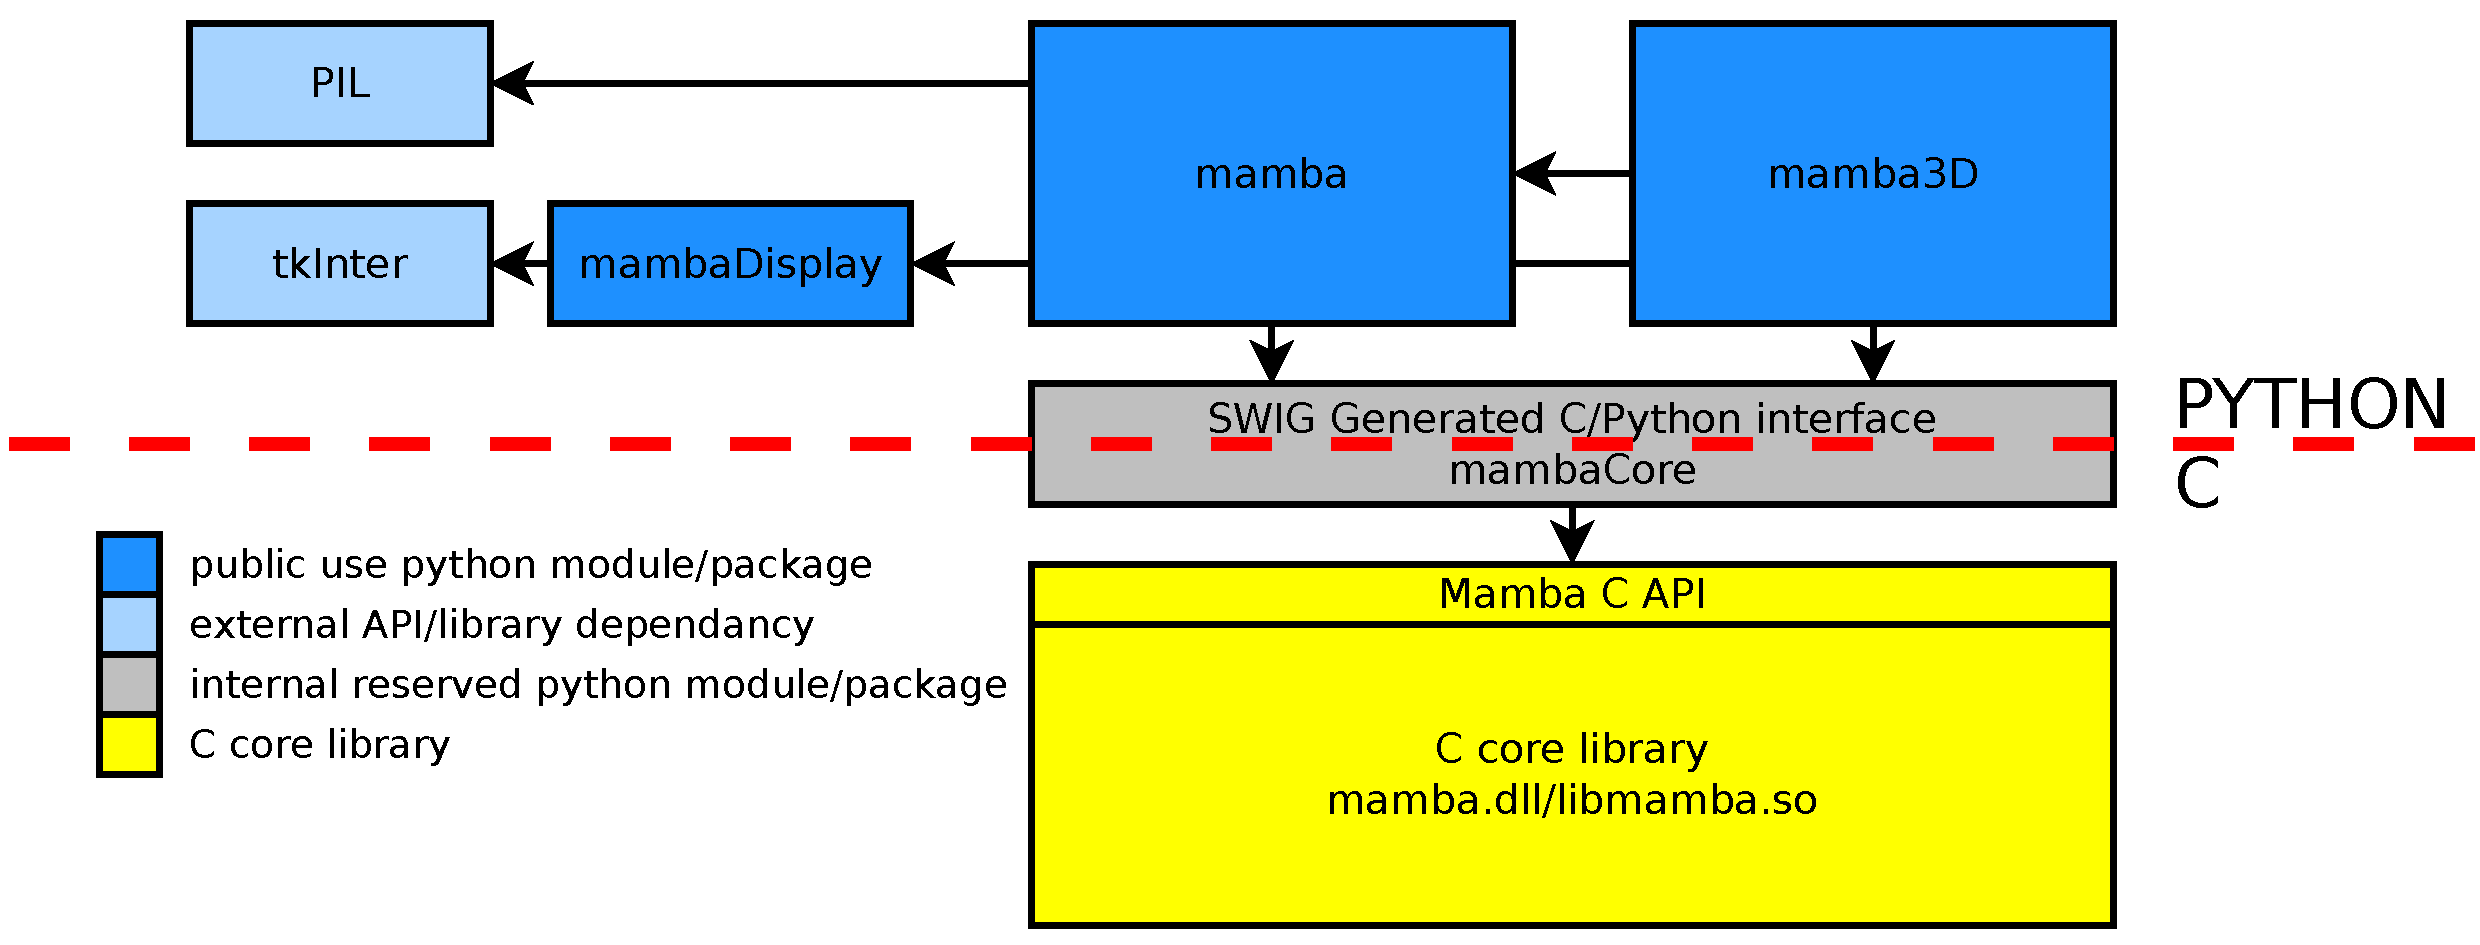
\includegraphics[width=0.7\textwidth]{figures/archi.pdf}
\caption{Library architecture layout}
\label{fig:archi_lay}
\end{figure}

As you already know, Mamba is programmed in C and Python. The C code implements
very basic functions. They are coded to be specific, fast and simple. Each 
function performs only one operation and do it the best it can. The C code is 
compiled to create the core library which is a collection of simple operations.

Simple Wrapper Interface Generator (SWIG) is used to create the interface 
between the C code and the Python code. This tool makes it easier to add new
functions inside the C part by automatically generating the Python wrapper
around it (Except for particular parameters).

The Python code is split into various packages. The mamba package is the 
main package. It implements the imageMb class that is the
central data structure of the library. This class is an extended, more Python
friendly, version of the data structure used to represent image data inside the
C core library. It also wraps the core functions to simplify them
and make them compatible with the imageMb class. The mamba3D package is the
equivalent of the mamba package for 3D images.

Because the C core library does not offer functions to read image files, Mamba
relies on the Python Imaging Library (Pillow) to do so. An internal module is used
to create an interface to Pillow that makes sure images are properly loaded and
converted to a format that is compatible with Mamba internal data representation.

The display capability is implemented by an internal module which relies on
Tkinter for windows and widgets creation.

This architecture is described in figure \ref{fig:archi_lay}.

\subsection{Creating your own displayer}
\label{cha:create_own_disp}

If your intent is to create your own display for Mamba image, you can create
a "displayer" class inheriting from the mambaDisplayer class described in the
mambaDisplay package. This class is actually an abstract class (or as close
as an abstract class that is allowed by Python). The mambaDisplay package
actually implements one child class of the mambaDisplayer called DftDisplayer.
Creating your own display will then look like this:

\lstset{language=Python}
\begin{lstlisting}
import mambaDisplay

# your own displayer (inherits from the generic displayer)
class YourOwnDisplayer(mambaDisplay.mambaDisplayer):
    ...
    
# Creating an instance of your displayer
your_displayer = YourOwnDisplayer()

# Setting up your displayer as the default
mambaDisplay.setDisplayer(your_displayer)
\end{lstlisting}

A "displayer" must implement various functionnalities to work correctly. The 
best way to create your own is to have a look at the default one in mambaDisplay.

\subsection{Vectorization}
\label{cha:vectorization}

Mamba C core library use vectorized computations to squeeze out better 
performance from your computer. Vectorization is achieved through the SSE2
instruction set available on all modern intel and AMD CPUs.

If you are planning to compile Mamba for other architectures you might want to
use the available equivalent instruction set. You can easily do this by modifying
the file mambaApi\_vector.h found in the src/mambaApi/include-private directory
in the sources.

Replace or add your own definition of the macros MB\_vec* using the appropriate
instruction set.

\subsection{Adding your own 3D grid}
\label{cha:create_grid3D}

To add your own grid, we recommand you have a look at the grids3D module in
the mamba3D package.

In it, you will find a class called \_grid3D that defines all the requested
methods that a grid must define to properly work in Mamba3D. Your own grid
will have to inherit from this class.

Of course, the best way to create your own grid is to copy and modify one
of the aforementioned grids (they can also be found in the grids3D module).

\subsection{Testing Mamba}
\label{cha:testing_mamba}

Mamba has a comprehensive set of tests designed to verify the appropriate
working of the library.

If you made some modifications on the library you may find useful to retest it
to prevent any unwanted regressions or to verify your modification did not break
the library.

Tests are located in the directory test of the sources. You can run the complete
set of tests by typing the following command in a terminal:

\texttt{python runTest.py -c -o test\_run.html -v 2}

Once the tests are done, you will find an HTML report with all the results in it.

The test runner makes use of coverage (see \url{https://pypi.python.org/pypi/coverage/3.7.1})
package to generate coverage information for the Python packages.

If you want more information regarding the test runner, you can type:

\texttt{python runTest.py -h}

\pagebreak

\appendix

\section{To go further}
\label{cha:to_go_further}
\subsection{Python websites}

Here is a list of Python related websites:

\begin{itemize}
\item \url{http://www.python.org}: The official Python website. You can download
it there, find documentation and other links for Python.
\item \url{http://docs.python.org/tutorial/}: The official Python tutorial.
\item \url{http://www.greenteapress.com/thinkpython/thinkCSpy/}: How to Think 
Like a Computer Scientist. A free book to learn computer science with Python
programming. Many translations are available.
\item \url{https://pypi.python.org/pypi/Pillow/}: The Pillow
website. You can download it, find documentation and source.
\item \url{http://wiki.python.org/moin/TkInter}: A wiki providing ressources
for the Tkinter library used in Mamba for display.
\item \url{http://www.pythonchallenge.com/}: An online puzzle game where you
will need to use Python to solve the riddles.
\end{itemize}

\subsection{Mathematical Morphology websites}

The list below presents websites where you will find courses, documentation and
other information related to mathematical morphology at large:

\begin{itemize}
\item \url{http://cmm.ensmp.fr/}: The Centre de Morphologie Math\'{e}matique
website. This Mines Paristech research laboratory was founded by Georges Matheron 
and Jean Serra, the pioneers of mathematical
morphology. Various publications are available with online courses.
\item \url{http://en.wikipedia.org/wiki/Mathematical_morphology}: The Wikipedia
page on mathematical morphology.
\end{itemize}

\subsection{Other mathematical morphology libraries}

If you are not happy with Mamba, here is a list of other mathematical morphology
libraries:

\begin{itemize}
\item \textsc{\textbf{Fulguro}}: A free library, released under LGPL, implementing
mathematical morphology and image processing functions. Coded in C with wrappers
for Python and Ruby. You can find it at \url{http://fulguro.sourceforge.net/}.
\item \textsc{\textbf{Morph-M}}: A proprietary library developed by the Centre
de Morphologie Math\'{e}matique. Morph-M is coded in C++ with a wrapper for
Python. More information can be found at \url{http://cmm.ensmp.fr/Morph-M/index_en.html}.
\end{itemize}

\pagebreak

\section{Coding rules and standards}
\label{rules}

Mamba is an open-source library and any contribution is welcome. In
order to help programmers, users and would be contributors, this appendix
presents the basic policy ruling the development of Mamba. It it our
vision, as its creators, of what is Mamba and where we want it to go
in the future. Anyone who wish to participate (by giving ideas, suggestions
or code) should read at least the policy section \ref{cha:Policy}.

\subsection{Policy}
\label{cha:Policy}

As you may already know, Mamba objective is to be a fast, simple,
portable and free (as in free speech but also as in free beer, this
being the case only because no one on Earth could afford it if we
had decided to sell it) mathematical morphology library. To cover
this purpose, a basic policy was decided by its creators.


\subsubsection{A Mathematical Morphology library}

Mamba is a mathematical morphology library only. It basically means
that there is no convolution, Fast Fourier Transform and such in it.
Only algorithms related to mathematical morphology may be present
in it.

This policy is one of the founding aspect of Mamba. The objective
it to prevent Mamba from dispersing itself into aspects that are not
related to its original purpose. We believe that there is already
enough good libraries out there to compute images using other techniques
than mathematical morphology and thus that there is no need for Mamba
to include them. On the other hand, as a Python library, Mamba can be
mixed efficiently with other image processing libraries also developped
in Python.


\subsubsection{Simple yet Fast}

Fast and simple can appear somehow contradictory as complex algorithms
may deliver faster performances. However, what we mean here is to
make sure Mamba is simple to use. As such, we believe that it is important
not to have to wait a very long time to get the result of your algorithm.
Mamba is meant to be used in research and education where you are
not always sure of your idea. Being able to rapidly evaluate the soundness
of an algorithm is also what will make Mamba simple to use. In other
words, the faster Mamba is, the simpler it becomes to try new ideas
with it. Moreover, Mamba is not only a simple educational software and
it can be used for solving real applications. Performance is even more
important in this case.

It seems also important for us to provide tools, inside Mamba, helping
users to \textquotedbl{}visualize\textquotedbl{} their ideas and thus
be able to easily assess their worthiness. As a result, Mamba comes
with a set of tools to fulfil this objective, the most visible being
the capability to see manipulated images in live. These tools are
a very important part of the library (equally in our eyes to the core
functions used in computations). Again, the objective is to provide
a simple framework for testing and trying new ideas in mathematical
morphology.


\subsubsection{Portable}

Mathematical morphology algorithms variety and diversity make it somehow
stupid to try to restrain their use to a very limited set of computers
and devices (or so we think). Thus the effort towards portability.


\subsubsection{... and Free}

Last but not least, as we hope Mamba will become a huge success and
help spread knowledge and use of mathematical morphology, we believe
it is important not to restrain its future users with a complex or
obscure license. Similarly, we think that a commercial license is inapropriate
for some of the intended audience of this library (students, university...)
and too complex for us to handle with others (industry, ...). Thus
we decided to license Mamba under a slightly modified version of the
X11 license (also known as the MIT license). This is one of the least
restrictive free license. Any contributor to Mamba will have to make
sure his contribution is licensed under a similar license (see \ref{cha:Licensing}).

\subsection{Programming}

\subsubsection{Languages}
\begin{itemize}
\item Mamba low level is written in C. 
\item Mamba high level is written in Python. 
\end{itemize}
This language choice is meant to cover the Mamba objective of being
a fast portable and easy to use library.

C choice for low-level answers the speed requirement and partly covers
the portability. Indeed, Mamba is meant to be portable to embedded
systems. Of course, the part written in C must be compilable on various
environmments (Windows, Unix ...) and for various processors (Pentium,
Core 2 Duo, ARM, ...).

Python choice is here to ensure easiness of use. As a high level language,
it makes it easier to develop programs and algorithms without taking
care of memory management, OS portability ... Other languages could
be used for high level but currently all the high level functionnalities
are written in Python. Of course, if you have the time and the need
to develop a high level interface in another language, feel free to
do so. However, maintaining multiple high level interfaces in different
languages may prove too much hassle so your high level interface may
not be integrated to the official Mamba distribution.

\subsubsection{Rules for C}

Three words can be used to sum up the philosophy of rules/standards
applying to Mamba C code.
\begin{itemize}
\item simplicity 
\item readability 
\item portability 
\end{itemize}
Simplicity means that your code must not try to answer all the problems
or to take into account all the possible situations. You should leave
the complexity to the high level interface (where generally it is
much easier to handle the real life situations).

Readability is a vague notion. Mainly, you have to make sure your
code is understandable. Comments, coherent naming, and so on are strongly
advised. More specific rules are :
\begin{itemize}
\item Use of english in comments is mandatory.
\item Function descriptions in comments use Doxygen style (see the documentation
section below for more details regarding documentation). At least all the 
exported functions must have a description.
\item Indentations are done using 4 spaces (no tabs, they are ugly because
they messed up when changing the editor). 
\item Functions and variables that are exported (visible by the exterior)
should begin with \textquotedbl{}MB\_\textquotedbl{}. 
\end{itemize}
Portability means that you should always take care to write your program
so that it will run on the greatest number of machines and equipments.
Of course this is not always feasable (particularly if you are going
very low level). Anyway, it simply means that if, for example, you
write an algorithm using SSE instructions of modern Intel/AMD processors,
you should also include your algorithm in standard C code (even if
that means it's excruciatingly slow).

\subsubsection{Rules for Python}
\label{cha:rules}

When coding in Python, you must take great care to make your code and the
various functionnalities you are implementing as simple to use as possible.

The rules presented here aim at defining good practices in the design of new 
Mamba operators in order that these operators be as general and usable as 
possible. Although these rules are not compulsory, you are advised to follow 
them if you wish to share your work. Presently, these rules concern mainly the
use of the very important arguments, edge, structuring element (se) and grid.
The use of input and output images is also considered.

It is also compulsory that your Python code be compatible with Python 2.x and
Python 3.x as it is the case for Mamba 2.

\paragraph{General rules for simplicity and readability}

The Python API is meant to be used easily by users regardless of their
proficiency at programming (of course they need to have a basic idea of what
they are doing).

Complexity is handled in the Python interface. Most of the time, C functions
only deal with image data and their depth. The Python code is in charge of 
calling the appropriate C function depending on the image depth it is 
dealing with. Thus the same function is used for binary, greyscale and 32-bit
images in Python and corresponds to three functions in C (one for
each depth). Complexity should only be handled in C if this makes
computations go significantly faster.

As for comments, you need to document each function that is meant
to be public with docstring. You should also begin your internal functions
with a \textquotedbl{}\_\textquotedbl{} that will tell Python that
it's an internal function (the same goes for global variables).

Every non internal function must provide a docstring explaining what it does,
its arguments and its output. Keep in mind that this docstring will be
automatically extracted to build the Python/Mamba reference documentation.

\paragraph{Rules for operators using 'grid' and/or 'se' as arguments}

The following five rules address particularly the use of the two arguments 'grid'
(grid used by the operator, hexagonal or square in 2D, cubic, face centered cubic or
centered cubic in 3D) and 'se' (structuring element
possibly used by the operator). As 'se' is always defined in association with a
specific grid, possible conflicts are at stake if these two arguments are used
in an antagonistic way inside the Mamba/Python scripts defining the operators.\par

\textbf{Rule n\textdegree{} 1}

When creating an operator or wrapping a C function, make sure that the grid, edge
and structuring element that may be given as argument have a default value
available when calling the Python function thus making it easier for
interactive sessions (by reducing the number of mandatory arguments).

For example, the following C function:
\lstset{language=C} 
\begin{lstlisting} 

MB_errcode MB_InfNbb(MB_Image *src,
                     MB_Image *srcdest,
                     Uint32 neighbors,
                     enum MB_grid_t grid,
                     enum MB_edgemode_t edge);
\end{lstlisting}
is wrapped in Python by the function :
\lstset{language=Python}
\begin{lstlisting} 
def infNeighbor(imIn, imInout, nb, grid=DEFAULT_GRID, edge=FILLED):
\end{lstlisting}

Information regarding edge and grid have default values in the Python module 
and thus do not need to be defined every time.

The same rule applies for structuring element, for example:
\begin{lstlisting} 
def dilate(imIn, imOut, n=1, se=DEFAULT_SE, edge=mamba.EMPTY):
\end{lstlisting}

\textbf{Rule n\textdegree{} 2}

If 'se' is passed as an argument in the operator, as 'se' is always associated
with a grid (for instance, SQUARE3X3 is defined on the square grid), internal
operators using a grid as argument must use this grid in their argument list. 
This 'grid' argument can be passed by means of the method getGrid() of the 
structuringElement class.\par

\emph{Example:}

buildOpen definition in module openClose.py (commented script):

\lstset{language=Python}
\begin{lstlisting}
def buildOpen(imIn, imOut, n=1, se=mC.DEFAULT_SE)
    """
    Performs an opening by reconstruction operation on image 'imIn' and puts the
    result in 'imOut'. 'n' controls the size of the opening. 'se' is passed as 
    default argument.
    """
    imWrk = mamba.imageMb(imIn)
    mamba.copy(imIn, imWrk)
    mC.erode(imIn, imOut, n, se=se)
    # 'se' is used by the erosion in the first step. You can use any structuring
    # element you wish to achieve this operation.
    mC.build(imWrk, imOut, grid=se.getGrid())
    # However, as you use a build operator in the second step and as this operator
    # depends on the grid in use, you must pass to it the grid associated with 
    # 'se'. This is done through the statement grid=se.getGrid() which assigns
    # to 'grid' the grid on which 'se' is defined.
\end{lstlisting}

\par
    
\textbf{Rule n\textdegree{} 3}

If 'grid' is used in the operator argument list, internal operators needing a 
structuring element 'se' as argument must explicitely define this 'se'. Make 
sure that 'se' is compatible with the 'grid' in use.\par 

\emph{Example:}

This example is not very useful, it is just to illustrate the rule...

\lstset{language=Python}
\begin{lstlisting}
def myOperator(imIn, imOut, grid=mamba.DEFAULT_GRID)
    """
    Performs an erosion of  'imIn' and puts the result in 'imOut'. 'grid' is
    passed as default argument. If 'grid' is hexagonal, the erosion must use an 
    hexagon and a square if 'grid' is square.
    """
    if grid == mamba.HEXAGONAL:
        se = mC.HEXAGON
    else:
        se = mC.SQUARE3X3
    # The structuring element 'se' is defined according to the grid in use.
    erode(imIn, imOut, se=se)
\end{lstlisting}

If you do not define explicitely the structuring element used by the erosion, 
DEFAULT\_SE will be used. However, you have no idea of  the status of this 
default structuring element (it could be DIAMOND for instance whereas the grid 
in use is hexagonal...).

You may argue that the definition of HEXAGON or SQUARE3X3 may also be changed by 
the user. This is true and this is the reason why it is not wise to modify the 
definition of standard structuring elements.

A lot of operators use what is called ``an elementary structuring element'' 
which is in fact the size 1 structuring element defined on the grid: if the grid 
is hexagonal, it corresponds to HEXAGON (in the standard definition) and to 
SQUARE3X3 if we deal with a square grid. In this situation, if you want to be 
sure to use an unmodified structuring element, you may proceed this way instead:

\lstset{language=Python}
\begin{lstlisting}
def myOperator(imIn, imOut, grid=mamba.DEFAULT_GRID)
    """
    Performs an erosion of  'imIn' and puts the result in 'imOut'. 'grid' is
    passed as default argument. If 'grid' is hexagonal, the erosion must use an 
    hexagon and a square if 'grid' is square.
    """
    se = structuringElement(mamba.getDirections(grid), grid):
    # The structuring element 'se' is  still defined according to the grid in 
    # use. Its definition uses directly the characteristics of the grid, that is
    # the list of all its directions (including direction 0) and the grid itself
    # which is necessarily associated to 'se'.
    erode(imIn, imOut, se=se)
\end{lstlisting}

\par
    
\textbf{Rule n\textdegree{} 4}
 
Using at the same time 'se' and 'grid' in an operator argument list is strictly 
forbidden. This practice is at best redondant (if 'se' and 'grid' are 
compatible), at worst dangerous and inconsistent.\par

It is obvious that, if this rule is not enforced, this will lead sooner or 
later to a ``grid and structuring element mess''. 

\par

\textbf{Rule n\textdegree{} 5}

It is possible that no argument ('grid' or 'se') be passed to an operator. This 
is allowed provided that no conflict is generated by this means. To achieve 
this, make sure that all internal operators use only either 'grid' or 'se'. If 
it is not the case (for instance, there exists in the definition script at 
least one operator requesting 'grid' and another one requesting 'se'), this 
situation is likely to produce conflicts and errors.

If no argument is passed, the operator will use DEFAULT\_SE or DEFAULT\_GRID 
defined outside its definition space (with a possible risk of conflicts).\par

\emph{Example:}

\lstset{language=Python}
\begin{lstlisting}
def alternateFilter(imIn, imOut, n):
    """
    Performs an alternate filter operation of size 'n' on image 'imIn' and puts
    the result in 'imOut'. If 'openFirst' is True, the filter begins with an
    opening, a closing otherwise.
    """
    if openFirst:
        mC.open(imOut, imOut, n)
        mC.close(imOut, imOut, n)
    else:
        mC.close(imOut, imOut, n)
        mC.open(imOut, imOut, n)
    # Neither open nor close need 'grid' in their arguments, but only 'se'. 
    # Therefore, as there is, in the definition of alternateFilter, no other
    # operator requesting 'grid', no conflict occurs and the structuring element
    # used by open and close will be DEFAULT_SE.
\end{lstlisting}

Although this rule is admitted, it is not wise in practice to apply it. Indeed, 
to be applied without risk, this rule states that all internal operators need 
only one argument, 'grid' or (exclusive) 'se', it is therefore more efficient 
and safe to systematically pass this argument in the operator argument list. 
This avoids later difficulties if the operator itself is used in the definition 
of more complex functions.

Thus, the following definition of 'alternateFilter' is safer and usable inside 
another definition:

\lstset{language=Python}
\begin{lstlisting}
def alternateFilter(imIn, imOut,n, se=mamba.DEFAULT_SE):
    """
    Performs an alternate filter operation of size 'n' on image 'imIn' and puts
    the result in 'imOut'. If 'openFirst' is True, the filter begins with an
    opening, a closing otherwise.
    """
    if openFirst:
        mC.open(imOut, imOut, n, se=se)
        mC.close(imOut, imOut, n, se=se)
    else:
        mC.close(imOut, imOut, n, se=se)
        mC.open(imOut, imOut, n, se=se)
\end{lstlisting}

These five rules are not mandatory and do not constitute a dogma. However, 
using them will avoid some nasty problems during your first steps with Mamba. 
They allow also a better applications sharing.

Most of the time, 'grid' and 'se' are passed in the argument list as default 
arguments (se=mC.DEFAULT\_SE and grid=mamba.DEFAULT\_GRID). This is very handy 
when you use Mamba operators in terminal/console mode to test ideas and to 
concatenate these operators in order to solve a problem. In this case, you 
generally work in a chosen environment, you know which grid you are using (the 
grid which is defined as default grid) and you control totally your structuring 
elements. For instance, if your grid is hexagonal, it is likely that your 
default structuring element is set to HEXAGON.

This interesting simplification when in interactive mode, is unacceptable when 
you define a new operator if you want to share it with other users. In this 
case, you do not control the environment anymore and you must make sure that 
this operator will be used according to your wishes. Therefore, it is of the 
outmost importance to correctly manage the 'grid' and 'se' arguments in your 
definition. 
 
\paragraph{Rules for input and output images}

You can define with Mamba new operators using one or more input image(s) and 
putting some results in one or more output image(s). An important programming 
rule is that your operators should be defined in such a way that the same image 
may be used both as input and output. This means that you must be aware to 
avoid to replace your input image by any output image prematurely. Indeed, if 
you do not take care of this rule, it is likely that, in most cases, no error 
will occur. However, your result will certainly be wrong.\par

\emph{Example:}

\lstset{language=Python}
\begin{lstlisting}
# First approach (bad one).

def myOper(imIn, imOut):
    """
    This operator computes  a very simple morphological gradient of imIn and
    puts the result in imOut.
    """
    imWrk = imageMb(imIn)
    dilate(imIn, imOut)
    erode(imIn, imWrk)
    sub(imOut, imWrk, imOut)
\end{lstlisting}

In this example, if imIn and imOut are identical, although no error is detected, 
the final result will be incorrect since, in the erode operator, imIn has been 
replaced by its dilation.

\lstset{language=Python}
\begin{lstlisting}
# Correct approach.

def myOper(imIn, imOut):
    """
    This operator computes  very simple morphological gradient of imIn and
    puts the result in imOut.
    """
    imWrk = imageMb(imIn)
    dilate(imIn, imWrk)
    erode(imIn, imOut)
    sub(imWrk, imOut, imOut)
\end{lstlisting}

In this case, imIn may possibly be overwritten after the erosion with no harmful 
consequences regarding the final result.

Here again, enforcing this rule makes your operators user friendly and their 
sharing is made easier. This rule can be implemented very easily by using 
intermediary working images in your definition and by copying the input imIn 
into the working image at the beginning of this definition. 


\paragraph{Rules for 'edge' argument in user-defined operators}

Contrary to 'grid' and 'se', it is generally neither necessary nor wise  to 
pass 'edge' in your operators arguments list. 

There is no default value in Mamba for 'edge'. The reason of this is that 'edge' 
is always used to impose specific behavior and properties to some operators. 
It is the case for instance with geodesic operators.  It is well known that non 
extensive geodesic operators need that 'edge' be defined as 'FILLED'. Obviously, 
for these operators, the edge setting is defined inside the operator definition 
and not at all in its argument list.

In fact, 'edge' allows to define two different contexts for your transformation 
depending on the way you consider the outer space, that is the space outside 
your image window.

If you consider that the outer space is empty, you are then in an euclidean 
context. In this configuration, 'edge' is defined as 'EMPTY' and the main 
consequence of this choice is that outer 'black' pixels may have some influence 
on the result of your transformation for inside pixels, in particular if your 
transformation is anti-extensive. Note that you could equally define the outer 
space as 'FILLED' in this context (and Mamba allows it without problem). 
However, this configuration is seldom used in practice, being considered as 
``unnatural'' (we prefer to imagine the outer space completely empty rather 
than totally filled!).

If you consider that you have no idea of the content of the outer space and, 
moreover, that you don't care of it, you are working in a geodesic context. 
Your image window is considered as a geodesic space and you do not have to take 
the outside pixels into account in your operator. This can be achieved by 
setting 'edge' accordingly in your definition. If  an extensive operator 
requesting the setting of 'edge' is called in the definition, 'edge' should be 
set to 'EMPTY'. Conversely, if the operator is anti-extensive, 'edge' should be 
set to 'FILLED'.

It is important to keep in mind the fact that an empty edge is NOT equivalent 
to an euclidean context and, conversely, that a filled edge is NOT equivalent 
to a geodesic context. This is the main reason why 'edge' should not be passed 
in your operator argument list.

The only case where this rule can be by-passed is when you know that the 
operator you are defining can be used in both contexts and that it produces a 
legitimate result (but possibly different). This is true for instance for the 
basic morphological operators: dilations, erosions, openings, closings, 
thinnings and thickenings. So, when defining another implementation of these 
basic transforms (this is perfectly allowed), it is nevertheless wise (if not 
compulsory) to pass 'edge' in the operator argument list.

\subsection{Documentation}

\subsubsection{In code}

As was explained in the programming section, documentation related
to code must take two forms :

For Python code, use docstring.

For C code, use Doxygen style.

You should indeed know that part of the actual documentation is created
automatically using these forms of documentation. The whole documentation
must be written in english.

\subsubsection{Other documents}

All the other documents existing to date were created using Latex.
Mamba comes with a specific Latex style that allows creating an homogeneous
set of documents (with header, code listing style, etc... coherent
between documents).

If you have an idea of documentation, we strongly advise you to use
Latex along with the Mamba style (which can be found in the source).
To use it, you simply need to create a directory texmf/tex/latex in
your \$HOME or wherever your Latex distribution may find it and add
the files mamba.sty and mamba\_logo\_white.png in it. We prefer Latex
because it makes it easier to track modifications inside our versioning
repository (Latex being text format and not binary).

For those of you who do not have Latex or who do not wish to use it,
we can accept documents in other formats provided you also give along
a PDF version of them (making sure that way that the document will
be readable by anyone).

And of course, whatever the format you choose, make sure your name
appears in the document.

\subsection{Testing}

Mamba is tested to ensure that it works properly and that it
implements correctly the mathematical morphology algorithms it uses.

Testing is performed in a specific environment. We tried to avoid verification
with test images because they are not easy to handle (often a lot of images to
store) and although they correctly reveal errors, they cannot be used to
identify and correct them. Another problem with test images is the production
of the expected result image and the insurance that it is correct.

There are two levels of testing:

\begin{itemize}
\item \textbf{\textsc{Basic C level operators/functions}} :
They are tested and verified as extensively as possible to ensure that they
are working properly and do not crash. The testing is performed by calling their
wrapping Python function. Algorithm soundness, edge effects,
grid effects, image depth acceptation, proper error handling are tested for every
C function.
\item \textbf{\textsc{Mathematical operators and other high-level Python functions}} :
These are tested less thoroughly as this is not a realistic task. Basic
algorithmic verification is performed. The idea is to cover all the Python code
(100\% code coverage) to make sure there is no typo.
\end{itemize}

Although we take great care of producing a bug free library, there is no way
for us to guarantee that. Tests are likely to have some blind spot. They are
mainly here to ensure a bottom line quality level and to prevent any regression.
If you have written some operators/functions and would like to add it into the
official Mamba release, we would be grateful if you could provide us with some
tests to verify them.

\subsection{Licensing}

\label{cha:Licensing}

For code contribution, make sure your work is licensed under a similar
license than the one covering Mamba. Here is a reminder of the license:

\vspace{0.5cm}

\begin{minipage}[c]{0.8\textwidth}%
 {\small Copyright (c) <2009>, <Your name here>}{\small \vspace{0.5cm} \par}

{\small Permission is hereby granted, free of charge, to any person
obtaining a copy of this software and associated documentation files
(the \textquotedbl{}Software\textquotedbl{}), to deal in the Software
without restriction, including without limitation the rights to use,
copy, modify, merge, publish, distribute, sublicense, and/or sell
copies of the Software, and to permit persons to whom the Software
is furnished to do so, subject to the following conditions: The above
copyright notice and this permission notice shall be included in all
copies or substantial portions of the Software.}{\small \vspace{0.5cm} \par}

{\small Except as contained in this notice, the names of the above copyright 
holders shall not be used in advertising or otherwise to promote the sale, use 
or other dealings in this Software without their prior written authorization.}
{\small \vspace{0.5cm} \par}

{\small THE SOFTWARE IS PROVIDED \textquotedbl{}AS IS\textquotedbl{},
WITHOUT WARRANTY OF ANY KIND, EXPRESS OR IMPLIED, INCLUDING BUT NOT
LIMITED TO THE WARRANTIES OF MERCHANTABILITY, FITNESS FOR A PARTICULAR
PURPOSE AND NONINFRINGEMENT. IN NO EVENT SHALL THE AUTHORS OR COPYRIGHT
HOLDERS BE LIABLE FOR ANY CLAIM, DAMAGES OR OTHER LIABILITY, WHETHER
IN AN ACTION OF CONTRACT, TORT OR OTHERWISE, ARISING FROM, OUT OF
OR IN CONNECTION WITH THE SOFTWARE OR THE USE OR OTHER DEALINGS IN
THE SOFTWARE. }%
\vspace{1cm}
\end{minipage}

Any similar license is appropriate (see X11 license, BSD license). Make sure
your license is compatible with GNU GPL and that it has NO copyleft
obligations (GPL is a copyleft license). If your license has a copyleft
obligation, we will not be able to add your code to the Mamba source. However
an optional package/module can be created that will let the user decide if the
copyleft obligation is a problem for her/him or not (see the mambaRealtime for
an example of this situation).

For documentation contributions, make sure that your work license
allows us to distribute it freely.

\subsection{Other contributions}

There are lot of things you could do for Mamba, even if your are not
a programmer or a writer.

First of all, you can give us feedback regarding the way you use Mamba.
Any comment, criticism or suggestion is welcome and will be taken
into consideration (as long as it does not infringe our policy).

\end{document}

